\chapter{Data sets}
In \refTab{tab:app_datasets} the DBS paths for all used data sets in the analysis are given. The data sets are divided into several primary data sets (PD), where the same-flavor data sets are used for the signal selection, the different-flavor data sets is used for the background prediction, and the $\ptmiss$ and $\HT$ data sets are used for the trigger efficiency measurement. Each group of data sets is subdivided into several run eras (B-H), and the 2017 version of reconstruction is used.

\begin{table}[htb]
 \centering
 \caption{DBS paths for the data sets used in the analysis. Their paths are similar, only the \texttt{PD} names vary. The dilepton data sets are used for the key analysis, whereas the $\HT$ and $\ptmiss$ data sets are used for the trigger efficiency measurement, see \refSec{sec:triggEff}.}
 \label{tab:app_datasets}
 \begin{tabular}{l|l}
  \hline
  \multirow{5}{*}{PDs}       & DoubleEG               \\
                             & DoubleMu               \\
                             & MuonEG                 \\
                             & HT                     \\
                             & MET                    \\\hline\hline
  \multirow{ 9}{*}{DBS path} & \verb|/PD/Run2016B-03Feb2017_ver2-v2/MINIAOD| \\
                             & \verb|/PD/Run2016C-03Feb2017-v1/MINIAOD| \\
                             & \verb|/PD/Run2016D-03Feb2017-v1/MINIAOD| \\
                             & \verb|/PD/Run2016E-03Feb2017-v1/MINIAOD| \\
                             & \verb|/PD/Run2016F-03Feb2017-v1/MINIAOD| \\
                             & \verb|/PD/Run2016G-03Feb2017-v1/MINIAOD| \\
                             & \verb|/PD/Run2016H-03Feb2017_ver2-v1/MINIAOD| \\
                             & \verb|/PD/Run2016H-03Feb2017_ver3-v1/MINIAOD| \\
  \hline
 \end{tabular}
\end{table}

\chapter{Simulated data sets}
\section*{Simulated standard model data sets}

In \refTab{tab:app_MCsets} DBS paths of the used SM simulated data sets are given together with their cross sections used for the normalization of the processes. In cases where NLO to NNLO k-factors are used, this is also stated in the table.

\begin{table}[tb]
 \centering
 \caption{All SM MC samples used in the analysis with their cross section. In the case k-factors are applied, they are given separately. The abbreviation \texttt{\{..\}} stands for \texttt{RunIISummer16MiniAODv2-PUMoriond17\_80X\_mcRun2\_asymptotic\_2016\_TrancheIV\_v6}. All samples are of the \texttt{MINIAODSIM} format. Additional k-factors to obtain NNLO cross sections for the $\PZ\PZ$ samples are applied per event in dependence of the $\pt$ of the diboson system.}
 \scriptsize
 \label{tab:app_MCsets}
 \begin{tabular}[width=\textwidth]{lll}
  \hline
  \normalsize{process}                             & \normalsize{data set}   & \normalsize{$\sigma\cdot k[\mathrm{pb}]$} \\\hline
  $\boldsymbol{\ttbar}$                            &                         &                                           \\
  $\ttbar\to\ell^{+}\PGn\cPqb+\ell^{-}\PAGn\cPaqb$ & \verb|/TTTo2L2Nu_Tune*_ttHtranche3_13TeV-powheg-pythia8/{..}-v1|  & $87.31$                                   \\
  $\boldsymbol{\ttbar\PGg}$                        &                         &                                           \\
  $\ttbar\PGg$                                     & \verb|/TTGamma_Dilept_Tune*_13TeV-amcatnlo-pythia8/{..}-v2| & $1.679$                                   \\
                                                   & \verb|/TTGamma_Hadronic_Tune*_13TeV-amcatnlo-pythia8/{..}-v2| & $3.482$                                   \\
                                                   & \verb|/TTGamma_SingleLeptFromT_Tune*_13TeV-amcatnlo-pythia8/{..}-v2| & $2.509$                                   \\
                                                   & \verb|/TTGamma_SingleLeptFromTbar_Tune*_13TeV-amcatnlo-pythia8/{..}-v2| & $2.509$                                   \\
  \textbf{Drell-Yan}                               &                         &                                           \\
  $\PZ/\PGg^{*}\to2\ell$                           & \verb|/DYJetsToLL_M-50_TuneCUETP8M1_13TeV-amcatnloFXFX-pythia8/{..}_ext2-v1| & $5765.4$                                  \\
  \textbf{diboson}                                 &                         &                                           \\
  $\PZ\PGg\to2\ell\PGg$                            & \verb|/ZGTo2LG_Tune*_13TeV-amcatnloFXFX-pythia8/{..}_ext1-v1| & $117.864\cdot1.06$                        \\
                                                   & \verb|/ZGTo2LG_Tune*_13TeV-amcatnloFXFX-pythia8/{..}-v1| & $117.864\cdot1.06$                        \\
                                                   & \verb|/ZGTo2LG_PtG-130_Tune*_13TeV-amcatnloFXFX-pythia8/{..}-v1| & $0.1404\cdot1.06$                         \\
  $\PW\PZ$                                         & \verb|/WZTo3LNu_Tune*_13TeV-powheg-pythia8/{..}-v1| & $4.42965\cdot1.109$                       \\
                                                   & \verb|/WZTo3LNu_Tune*_13TeV-powheg-pythia8/{..}_ext1-v3| & $4.42965\cdot1.109$                       \\
  $\PZ\PZ\to2\ell2\PGn$                            & \verb|/ZZTo2L2Nu_13TeV_powheg_pythia8_ext1/{..}-v1| & $0.5644\cdot k(\pt^{ZZ})$                 \\
                                                   & \verb|/ZZTo2L2Nu_13TeV_powheg_pythia8/{..}-v1| & $0.5644\cdot k(\pt^{ZZ})$                 \\
  $\PZ\PZ\to4\ell$                                 & \verb|/ZZTo4L_13TeV_powheg_pythia8/{..}-v1| & $1.212\cdot k(\pt^{ZZ})$                  \\
                                                   & \verb|/ZZTo4L_13TeV_powheg_pythia8_ext1/{..}-v1| & $1.212\cdot k(\pt^{ZZ})$                  \\
  $\PW\PW\to2\ell2\PGn$                            & \verb|/WWTo2L2Nu_13TeV-powheg/{..}-v1| & $12.178$                                  \\
  $\PW\Pg\to\ell\PGn\Pg$                           & \verb|/WGToLNuG_Tune*_13TeV-amcatnloFXFX-pythia8/{..}_ext3-v1| & $489$                                     \\
  \textbf{W+jets}                                  &                         &                                           \\
  $\PW+jets$                                       & \verb|/WJetsToLNu_Tune*_13TeV-amcatnloFXFX-pythia8/{..}_ext2-v2| & $61526.7$                                 \\
                                                   & \verb|/WJetsToLNu_Tune*_13TeV-amcatnloFXFX-pythia8/{..}-v1| & $61526.7$                                 \\
  \textbf{triboson}                                &                         &                                           \\
  $\PW\PW\Pg$                                      & \verb|/WWG_Tune*_13TeV-amcatnlo-pythia8/{..}_ext1-v1| & $0.2147$                                  \\
  $\PW\PZ\Pg$                                      & \verb|/WZG_Tune*_13TeV-amcatnlo-pythia8/{..}-v1| & $0.04123$                                 \\
  \textbf{single top}                              &                         &                                           \\
  $\PWp\to\cPqt\cPaqb$                             & \verb|/ST_s-channel_4f_leptonDecays_13TeV-amcatnlo-pythia8_*/{..}-v1| & $3.36$                                    \\
  $\cPq\cPaqb\to\cPq^{'}\cPaqt$                    & \verb|/ST_t-channel_antitop_4f_incl*Decays_13TeV-powhegV2-*-pythia8_*/{..}-v1| & $80.95$                                   \\
  $\cPq\cPqb\to\cPq^{'}\cPqt$                      & \verb|/ST_t-channel_top_4f_incl*Decays_13TeV-powhegV2-*-pythia8_*/{..}-v1| & $136.02$                                  \\
  $\cPaqb\to\PWp\cPaqt$                            & \verb|/ST_tW_antitop_5f_NoFullyHadronicDecays_13TeV-powheg_*/{..}_ext1-v1| & $11.7$                                    \\
  $\cPqb\to\PWm\cPqt$                              & \verb|/ST_tW_top_5f_NoFullyHadronicDecays_13TeV-powheg_*/{..}_ext1-v1| & $11.7$                                    \\
  \hline
 \end{tabular}
\end{table}

\FloatBarrier
\section*{Simulated SUSY data sets}
In \refTab{tab:app_signalsets} the DBS paths for the used signal simulated data sets are given. Because in each signal data set very different paramater masses are used in the generation, many cross sections are used for the rescaling of the simulation, and are not quoted in the table.

\begin{table}[tb]
 \centering
 \caption{All SUSY MC samples used in the analysis. The abbreviation \texttt{\{..\}} stands for \texttt{80X\_mcRun2\_asymptotic\_2016}. All samples are of the \texttt{MINIAODSIM} format.}
 \scriptsize
 \label{tab:app_signalsets}
 \begin{tabular}[width=\textwidth]{ll}
  \hline
  \normalsize{signal}             & \normalsize{data set}   \\\hline
  \textbf{electroweak production} &                         \\
  TChiNG                          & \verb|/SMS-TChiNG_BF50N50G_*/RunIISpring16MiniAODv2-PUSpring16Fast_{..}_miniAODv2_v0-v1| \\
  GMSB                            & \verb|/GMSB_GravitinoLSP_N1decays_*/RunIISummer16MiniAODv2-PUSummer16Fast_{..}_TrancheIV_v6-v1| \\
  \textbf{strong production}      &                         \\
  T5bbbbZG                        & \verb|/SMS-T5bbbbZg_*/RunIISummer16MiniAODv2-PUSummer16Fast_{..}_TrancheIV_v6-v2| \\
  \hline
 \end{tabular}
\end{table}

\FloatBarrier

\chapter{Signal properties}\label{sec:app_signal}
In this chapter, properties of the three signal models considered in the interpretation of this analysis are given.
\section*{Signal cross section}
The production cross sections for the two simplified models and the GMSB model are shown in \refFig{fig:app_xsec} in the corresponding parameter mass planes. For the GMSB model, the production cross section depends only on the wino mass, since $\PSGczDo\PSGcpmDo$ and $\PSGcmpDo\PSGcpmDo$ are by the far the most dominant production channels and both the chargino and the neutralino are wino-like, see \refSec{sec:SMS}. Since in the \texttt{T5bbbbZG} SMS only gluino production is considered, the gluino mass determines the cross section. In the \texttt{TChiZG} SMS, only neutralino-chargino and chargino-chargino production is assumed.
\begin{figure}
 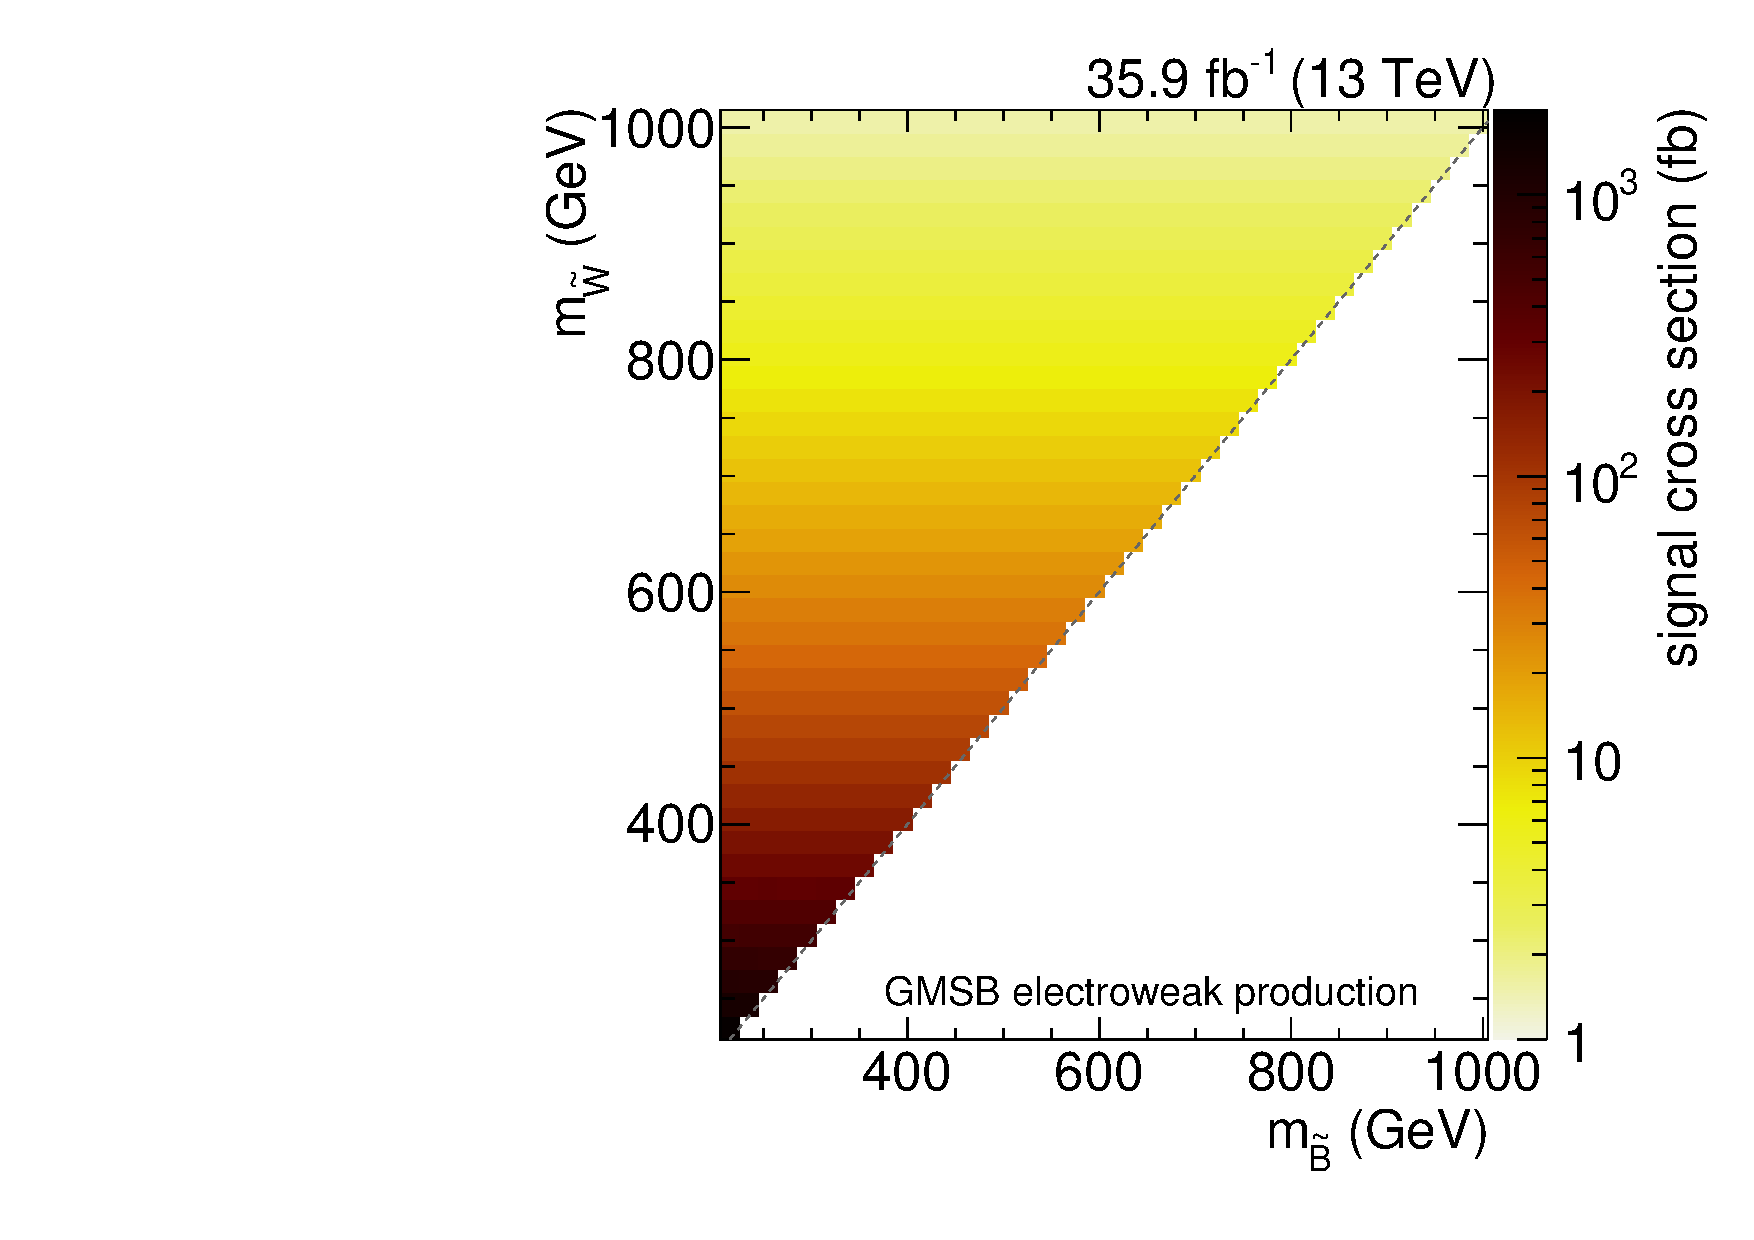
\includegraphics[width=\pairwidth]{figures/acceptance/GMSB_xsec_log}
 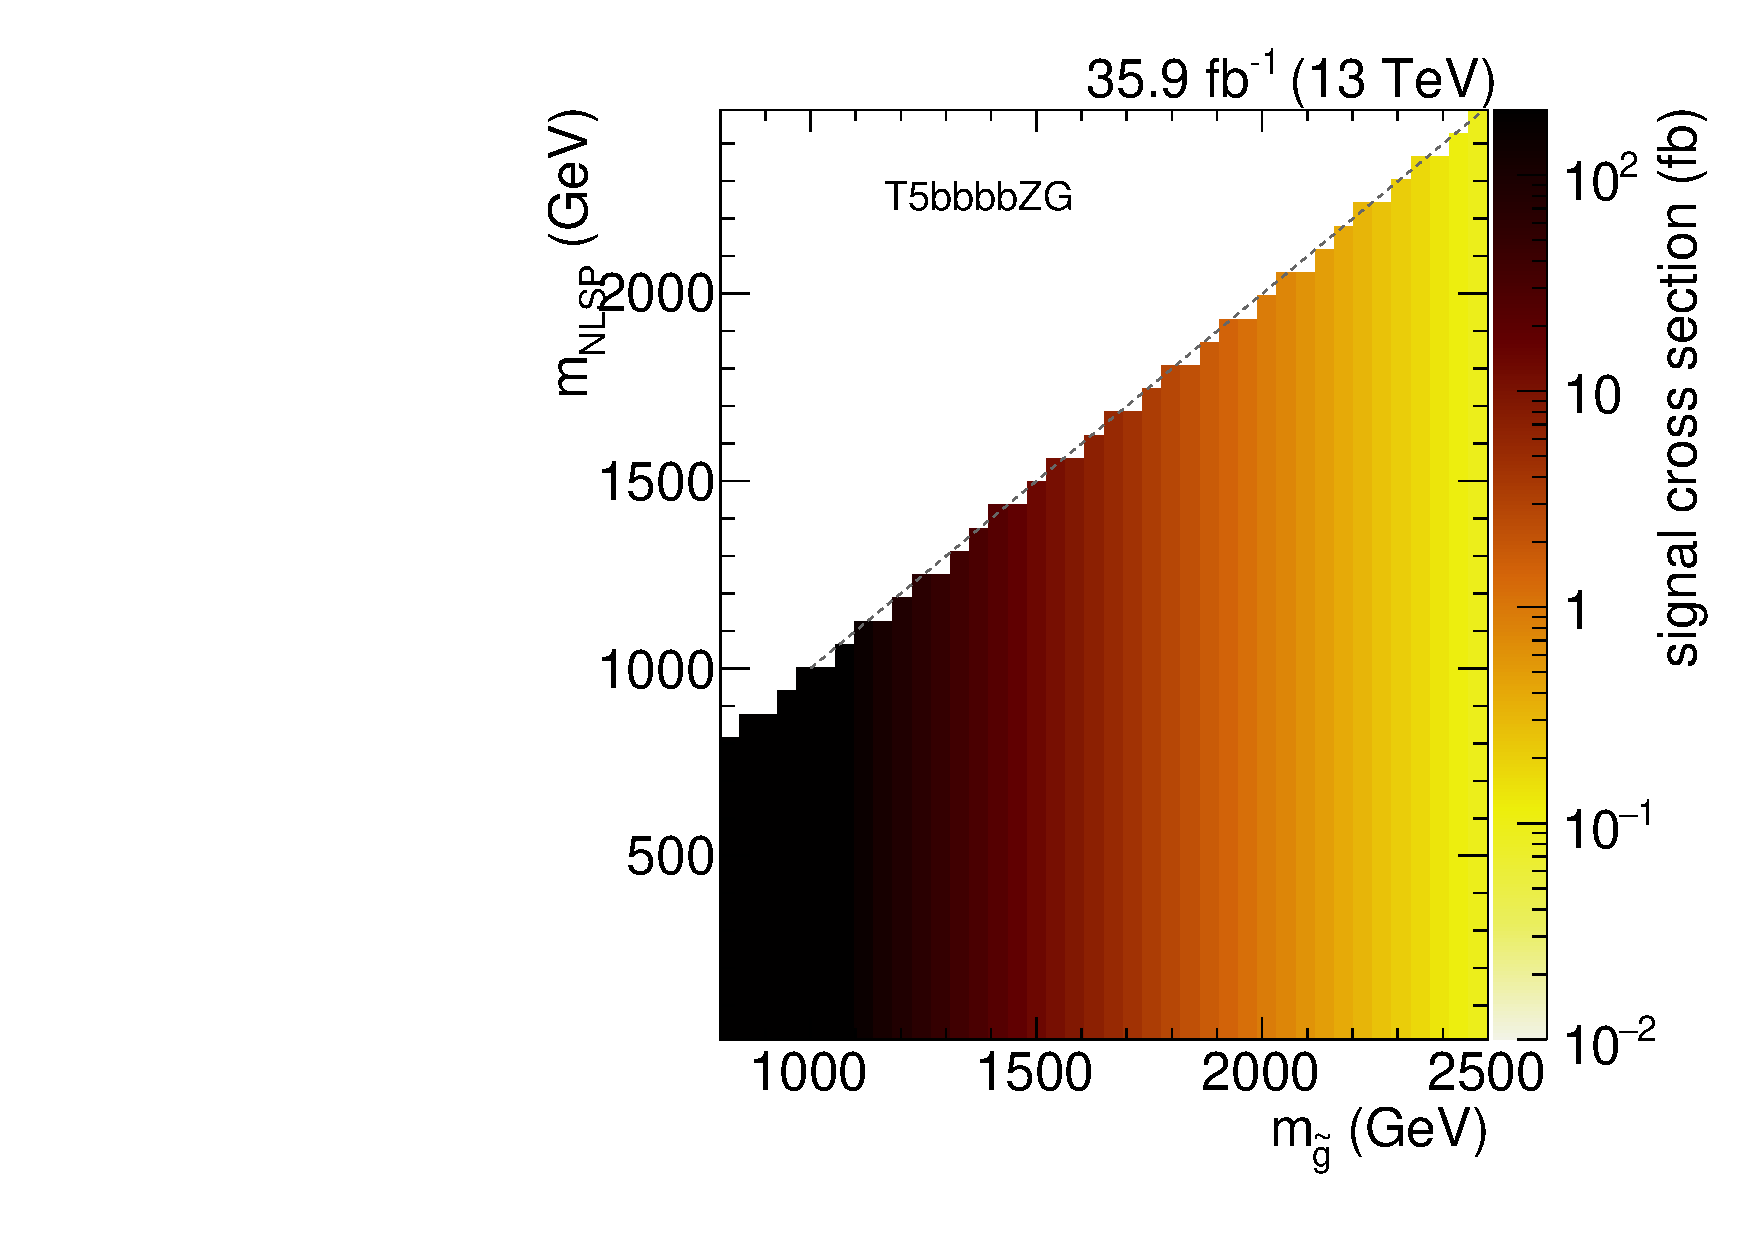
\includegraphics[width=\pairwidth]{figures/acceptance/T5bbbbZg_xsec_log}
 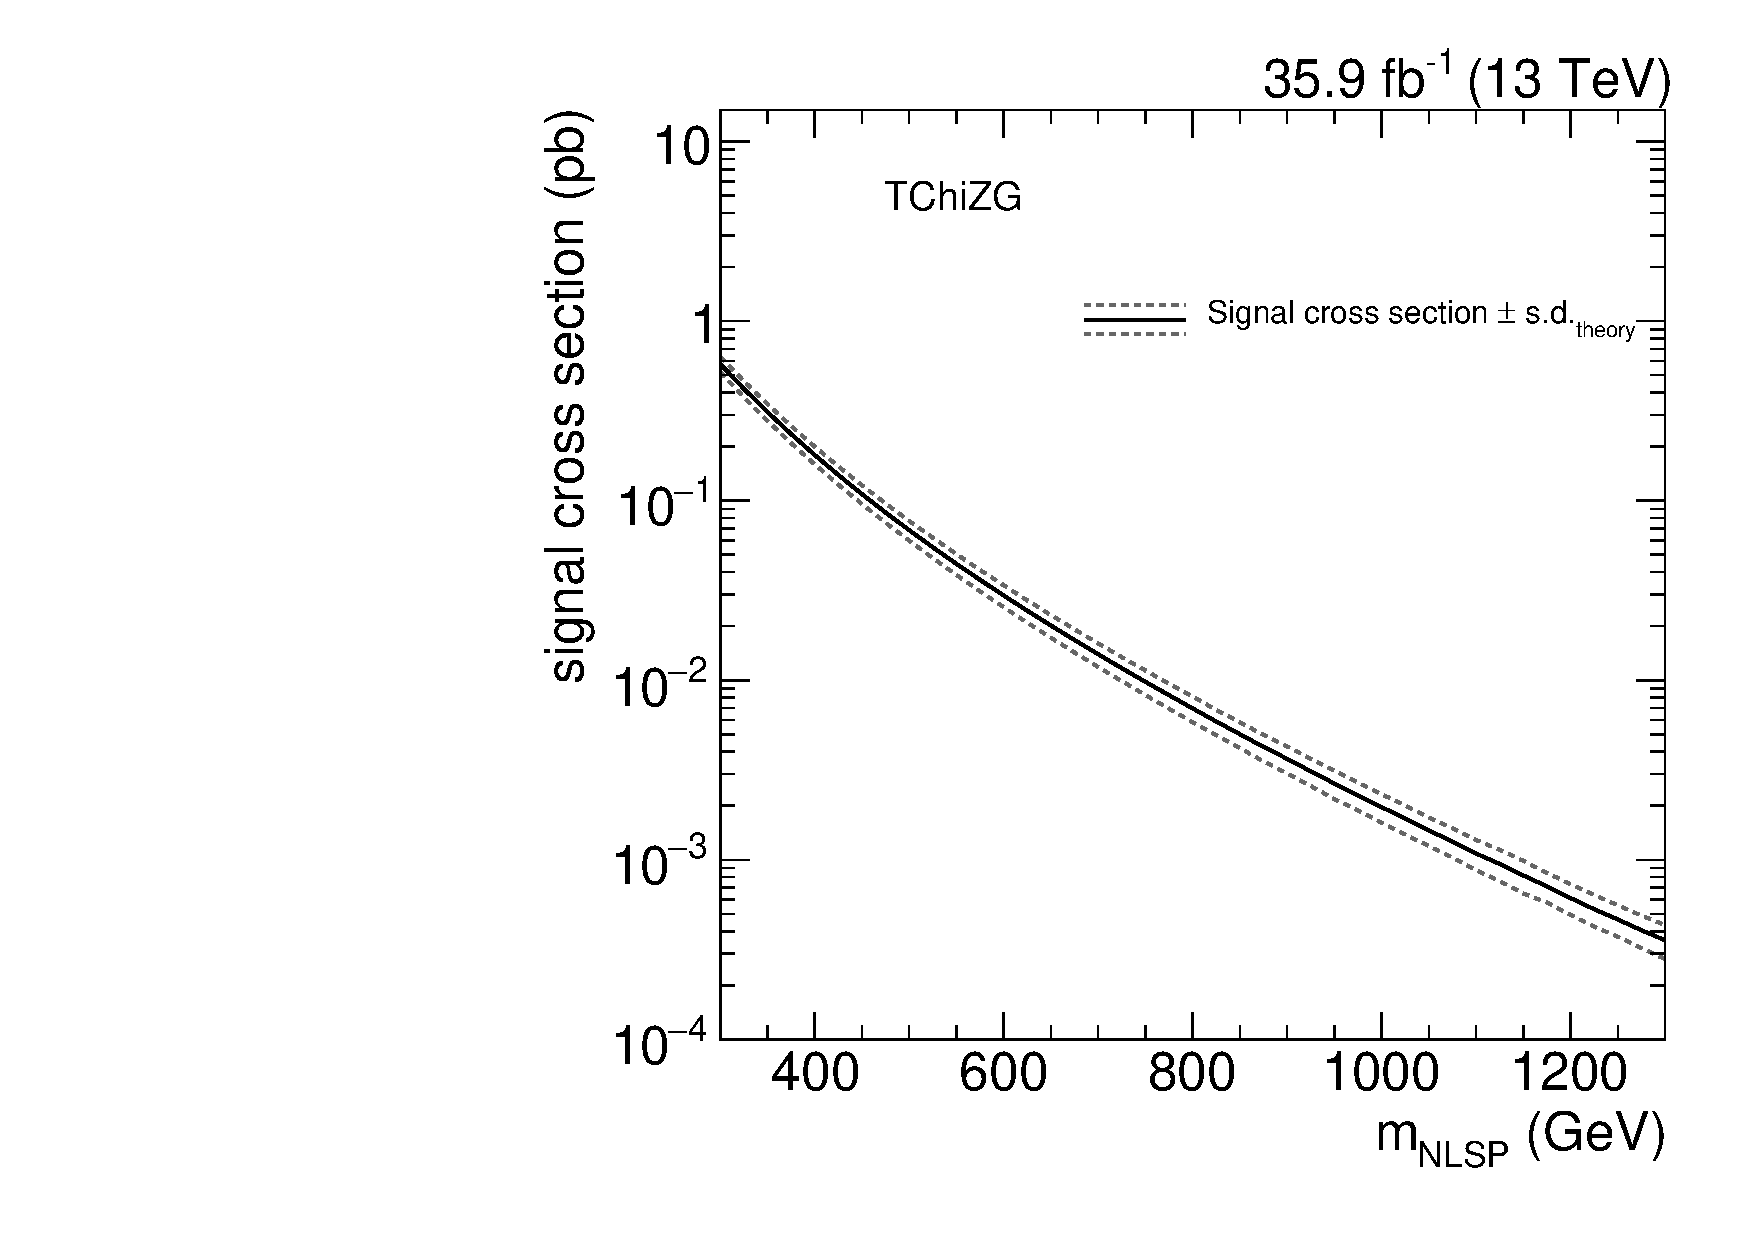
\includegraphics[width=\pairwidth]{figures/acceptance/TChiNG_XSECGRAPH}
 \caption{In the upper row, production cross sections for the GMSB model (left) and \texttt{T5bbbbZG} SMS are given in the $m(\widetilde{B})$ - $m(\widetilde{W})$ and $m(\mathrm{NLSP})$ - $m(\tilde{g})$ mass plane, respectively. The considered production cross section for the \texttt{TChiZG} model is given in the lower row.}
 \label{fig:app_xsec}
\end{figure}
\FloatBarrier

\section*{Event selection acceptance}
The total event selection acceptances, see \refSec{chap:results} for the definition, are shown in \refFig{fig:app_acceptance} for all three signal models. They are in the order of $\mathcal{O}(1\%)$, slighlty depending on the sparticle masses. In general, for higher sparticle masses the acceptance increases, since the final tate particles carry much more energy and the probability to be selected in the SR is larger. For low NLSP masses in case of the \texttt{T5bbbbZG} SMS, the acceptance decreases due to the $\mtTwo$ requirement of $100\GeV$. The acceptance is enhanced for the GMSB model, if the mass difference between the wino and bino is approximately $90\GeV$, because additional $\PZ$ bosons are produced in decays of sparticles in th cascades.
\begin{figure}
 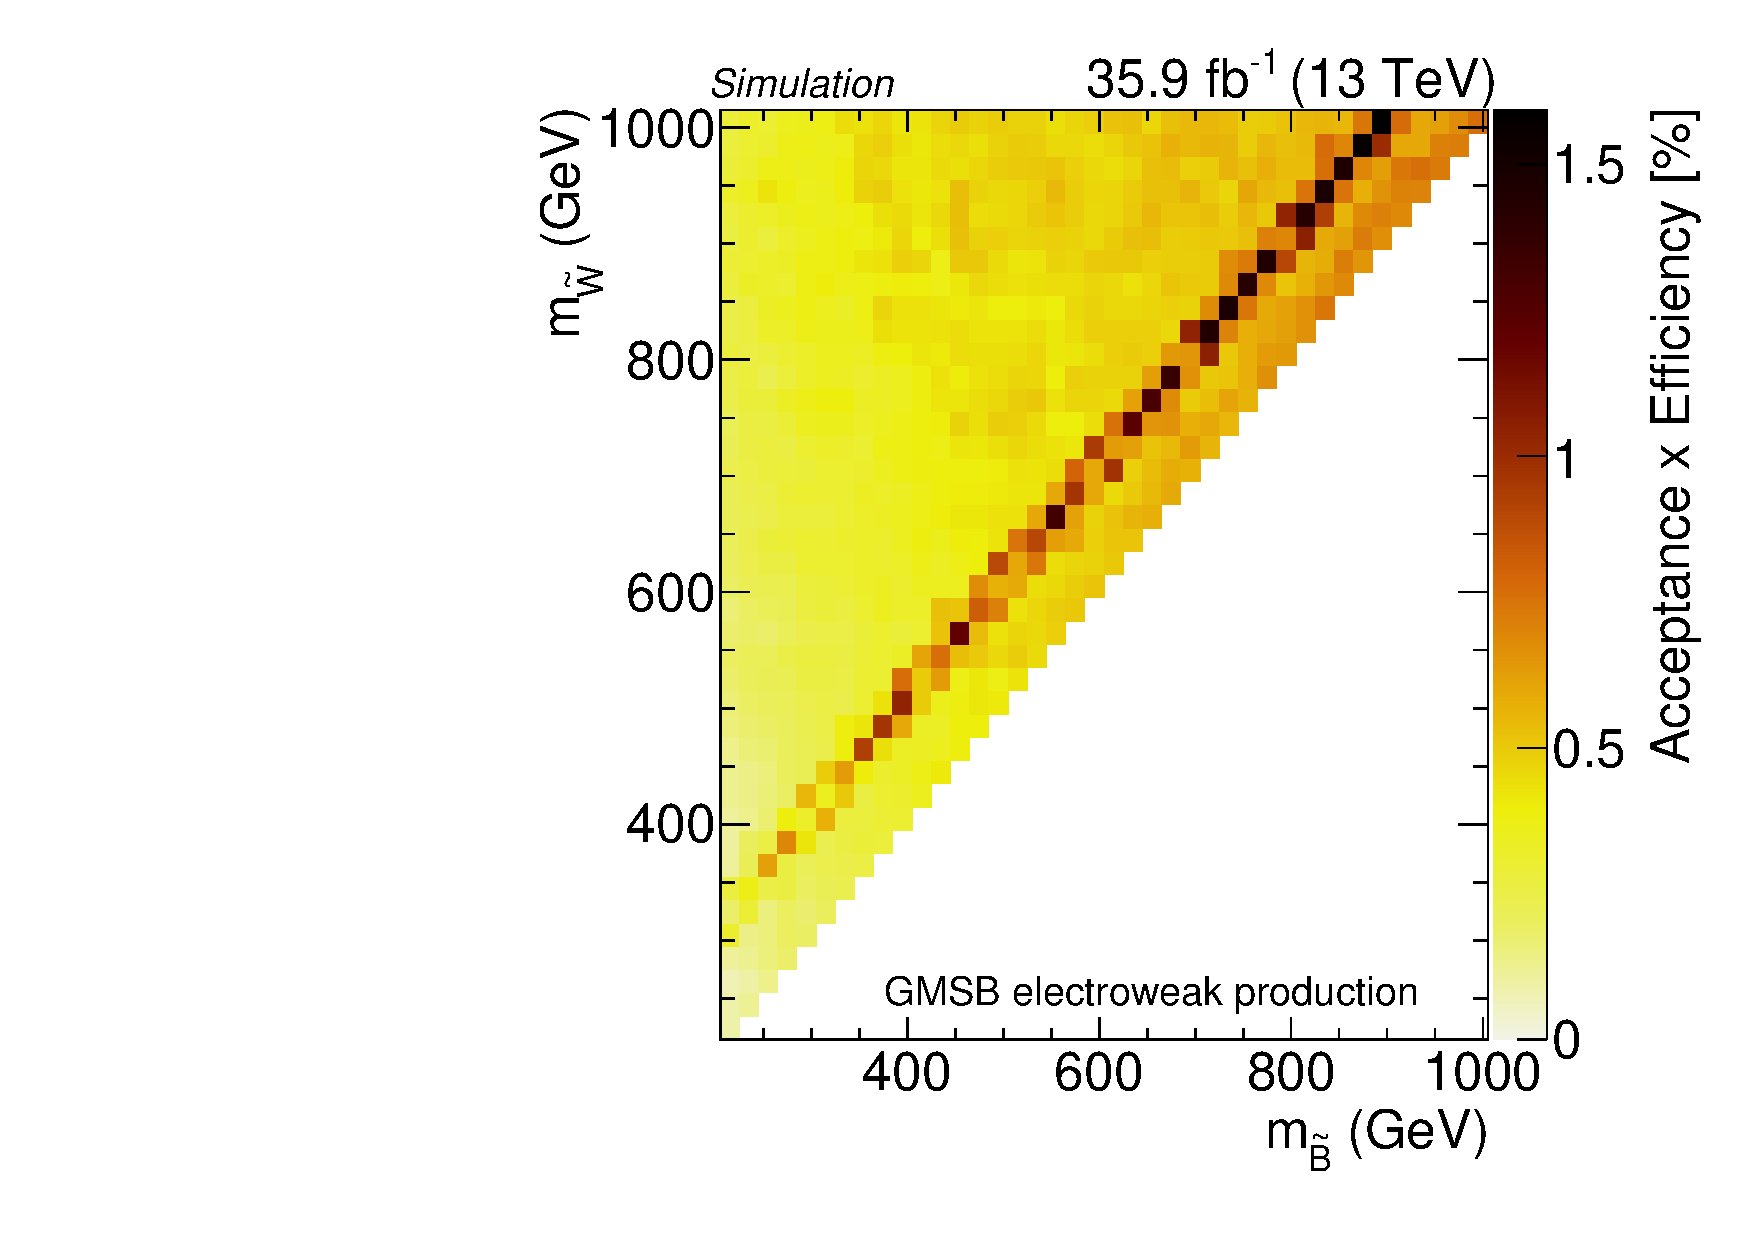
\includegraphics[width=\pairwidth]{figures/acceptance/gmsb}
 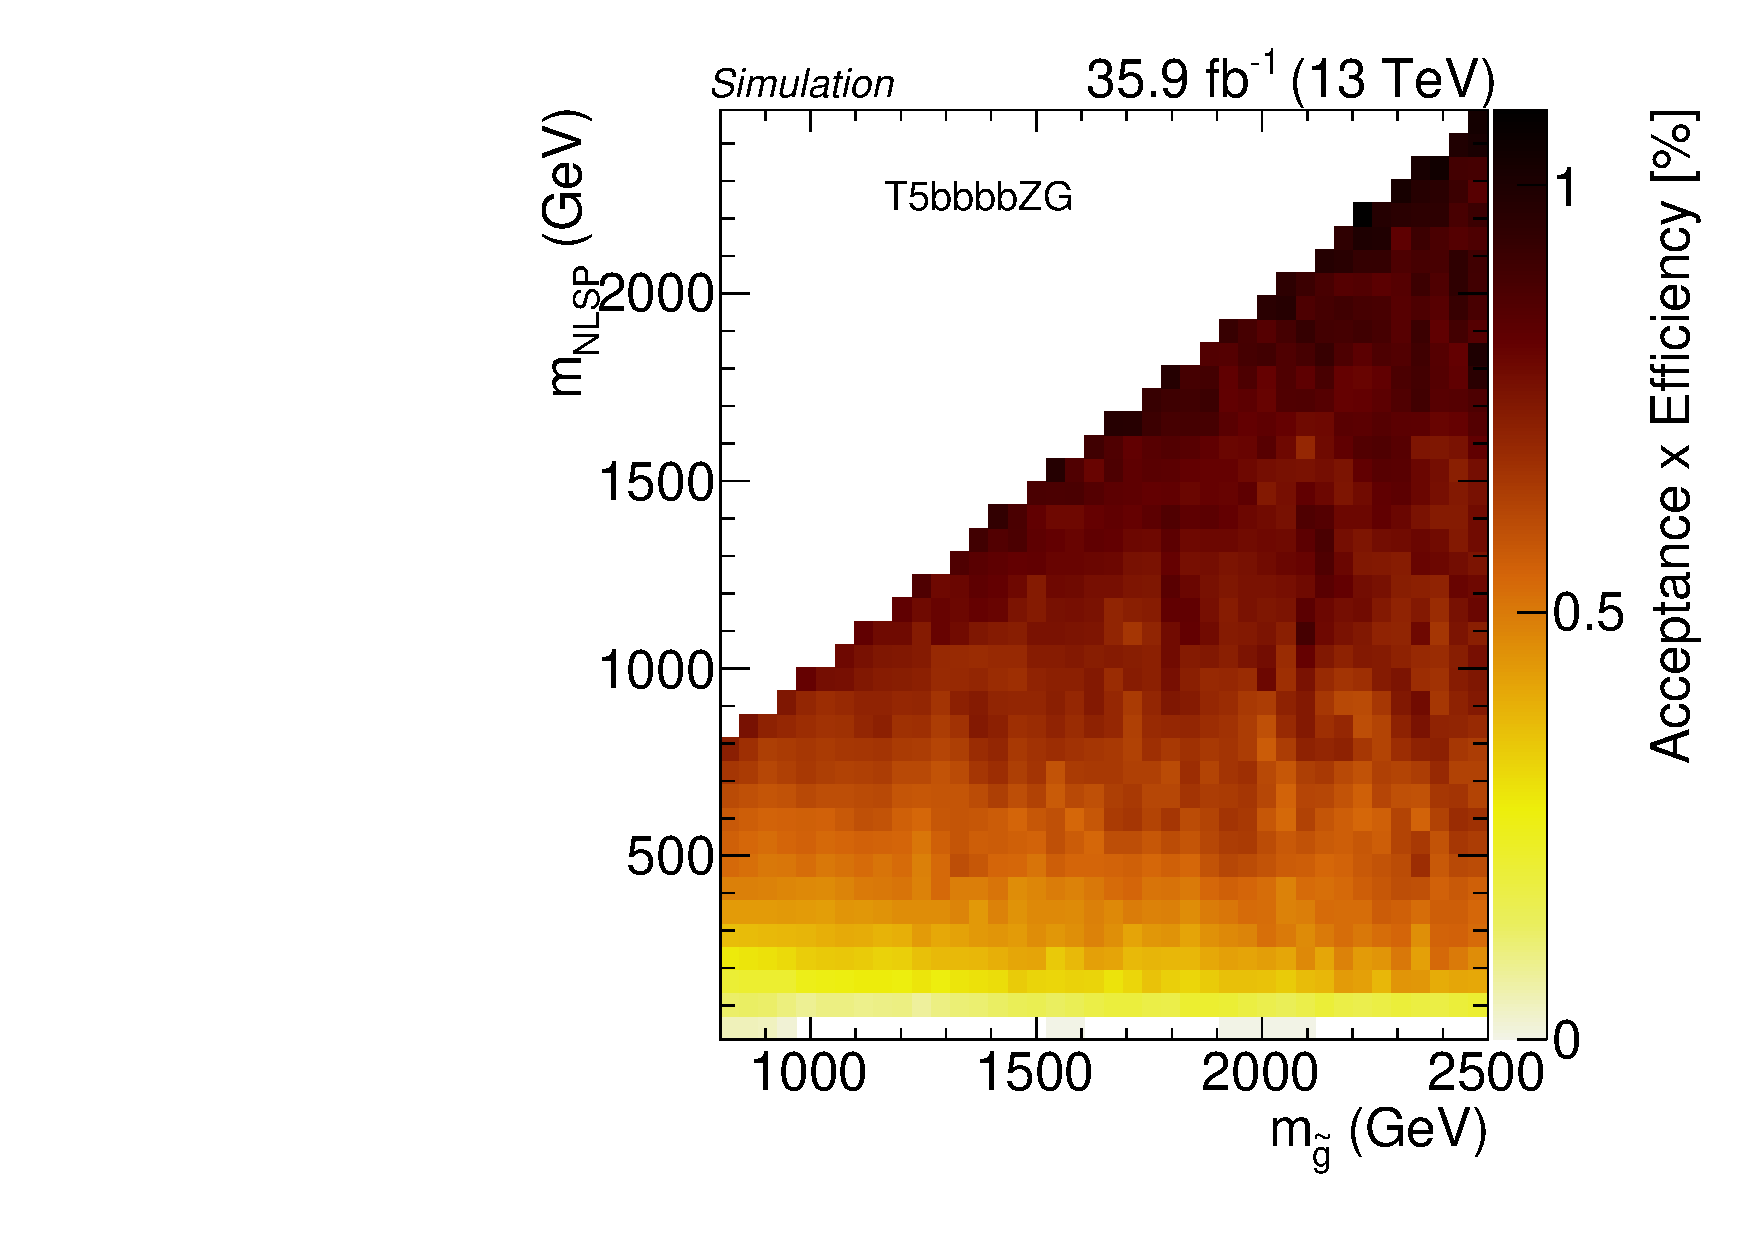
\includegraphics[width=\pairwidth]{figures/acceptance/t5zg}
 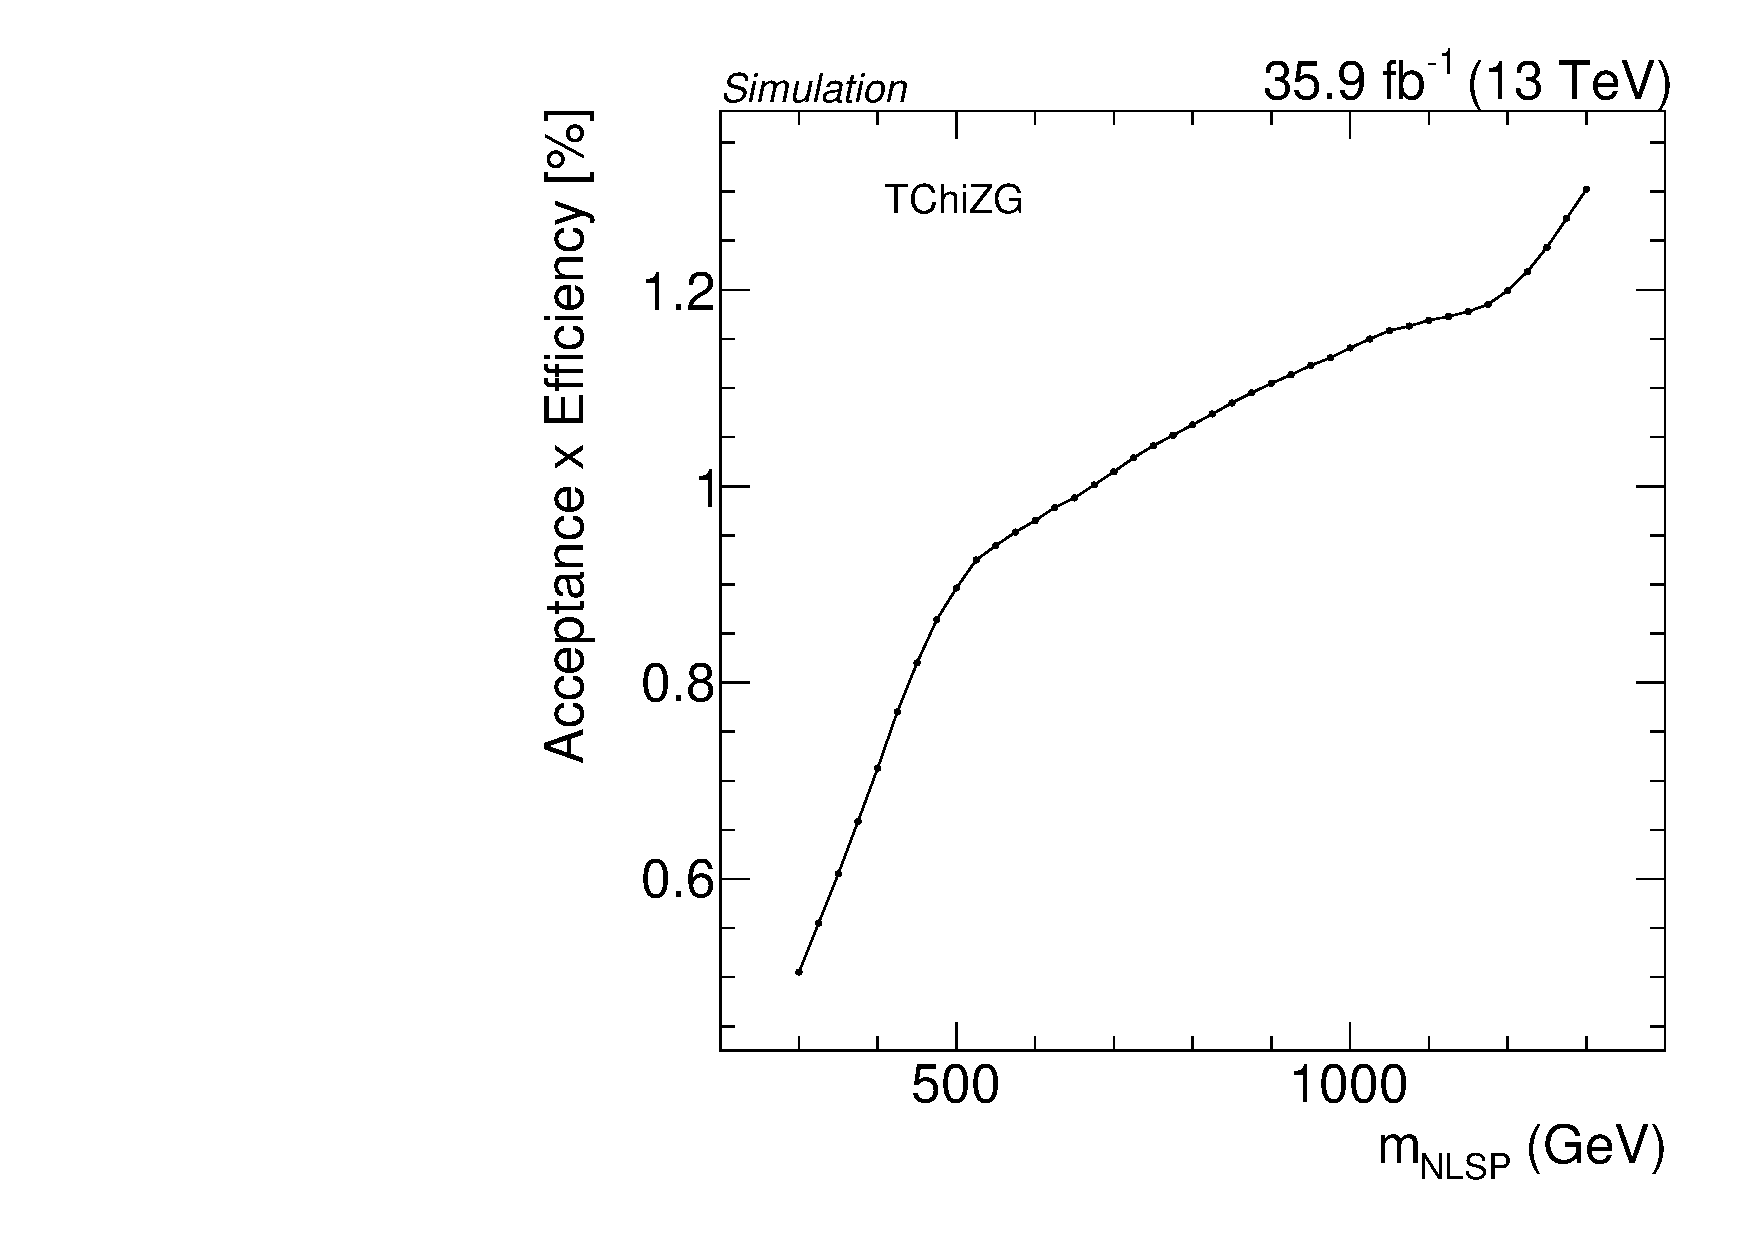
\includegraphics[width=\pairwidth]{figures/acceptance/tching}
 \caption{In the upper row, the event selection acceptance for the GMSB model (left) and \texttt{T5bbbbZG} SMS is shown in the $m(\widetilde{B})$ - $m(\widetilde{W})$ and $m(\mathrm{NLSP})$ - $m(\tilde{g})$ mass plane, respectively. The acceptance for the \texttt{TChiZG} model is given in the lower row.}
 \label{fig:app_acceptance}
\end{figure}
\FloatBarrier

\chapter{Trigger paths}

In Tables \oldref*{tab:app_trigger1} and \oldref*{tab:app_trigger2} all HLT trigger paths used in the analysis are quoted. The trigger paths in the first table are relevant for the signal event selection and the background prediction, while the HLT paths stated in the second table are needed for the trigger efficiency measurement.

\begin{table}[htb]
 % \begin{table*}[htb]
 \centering
 \caption{Trigger paths used for the signal and control region event selection.}
 \normalsize
 \label{tab:app_trigger1}
 \begin{tabular}[width=\textwidth]{l}
  \hline
  \normalsize{\textbf{dielectron trigger}}    \\
  \verb|HLT_Ele17_Ele12_CaloIdL_TrackIdL_IsoVL_DZ_v*|                     \\
  \verb|HLT_Ele23_Ele12_CaloIdL_TrackIdL_IsoVL_DZ_v*|                     \\
  \verb|HLT_DoubleEle33_CaloIdL_GsfTrkIdVL_v*|                     \\
  \verb|HLT_DoubleEle33_CaloIdL_GsfTrkIdVL_MW_v*|                     \\
  \normalsize{\textbf{dimuon trigger}}        \\
  \verb|HLT_Mu17_TrkIsoVVL_Mu8_TrkIsoVVL_v*|                     \\
  \verb|HLT_Mu17_TrkIsoVVL_TkMu8_TrkIsoVVL_v*|                     \\
  \verb|HLT_Mu17_TrkIsoVVL_Mu8_TrkIsoVVL_DZ_v*|                     \\
  \verb|HLT_Mu17_TrkIsoVVL_TkMu8_TrkIsoVVL_DZ_v*|                     \\
  \verb|HLT_TkMu17_TrkIsoVVL_TkMu8_TrkIsoVVL_DZ_v*|                     \\
  \verb|HLT_Mu27_TkMu8_v*|                     \\
  \verb|HLT_Mu30_TkMu11_v*|                     \\
  \normalsize{\textbf{electron-muon trigger}} \\
  \verb|HLT_Mu17_TrkIsoVVL_Ele12_CaloIdL_TrackIdL_IsoVL_v*|                     \\
  \verb|HLT_Mu23_TrkIsoVVL_Ele8_CaloIdL_TrackIdL_IsoVL_v*|                     \\
  \verb|HLT_Mu23_TrkIsoVVL_Ele8_CaloIdL_TrackIdL_IsoVL_DZ_v*|                     \\
  \verb|HLT_Mu23_TrkIsoVVL_Ele12_CaloIdL_TrackIdL_IsoVL_v*|                     \\
  \verb|HLT_Mu23_TrkIsoVVL_Ele12_CaloIdL_TrackIdL_IsoVL_DZ_v*|                     \\
  \verb|HLT_Mu8_TrkIsoVVL_Ele17_CaloIdL_TrackIdL_IsoVL_v*|                     \\
  \verb|HLT_Mu8_TrkIsoVVL_Ele23_CaloIdL_TrackIdL_IsoVL_v*|                     \\
  \verb|HLT_Mu8_TrkIsoVVL_Ele23_CaloIdL_TrackIdL_IsoVL_DZ_v*|                     \\
  \verb|HLT_Mu12_TrkIsoVVL_Ele23_CaloIdL_TrackIdL_IsoVL_v*|                     \\
  \verb|HLT_Mu12_TrkIsoVVL_Ele23_CaloIdL_TrackIdL_IsoVL_DZ_v*|                     \\
  \verb|HLT_Mu30_Ele30_CaloIdL_GsfTrkIdVL_v*|                     \\
  \verb|HLT_Mu33_Ele33_CaloIdL_GsfTrkIdVL_v*|                     \\
  \hline
 \end{tabular}
\end{table}




\begin{table}[htb]
 % \begin{table*}[htb]
 \centering
 \caption{Trigger paths used for the trigger efficiency measurements.}
 \normalsize
 \label{tab:app_trigger2}
 \begin{tabular}[width=\textwidth]{l}
  \hline
  \normalsize{\textbf{HT trigger}}  \\
  \verb|HLT_PFHT200_v*|           \\
  \verb|HLT_PFHT250_v*|           \\
  \verb|HLT_PFHT300_v*|           \\
  \verb|HLT_PFHT350_v*|           \\
  \verb|HLT_PFHT400_v*|           \\
  \verb|HLT_PFHT475_v*|           \\
  \verb|HLT_PFHT600_v*|           \\
  \verb|HLT_PFHT650_v*|           \\
  \verb|HLT_PFHT800_v*|           \\
  \normalsize{\textbf{MET trigger}} \\
  \verb|HLT_PFMET110_PFMHT110_IDTight_v*|           \\
  \verb|HLT_PFMET120_PFMHT120_IDTight_v*|           \\
  \verb|HLT_PFMET170_NoiseCleaned_v   *|           \\
  \verb|HLT_PFMET170_HBHECleaned_v*|           \\
  \verb|HLT_PFMET170_JetIdCleaned_v*|           \\
  \verb|HLT_PFMET170_NotCleaned_v*|           \\
  \verb|HLT_PFMET300_v*|           \\
  \verb|HLT_PFMET400_v*|           \\
  \verb|HLT_PFMET500_v*|           \\
  \verb|HLT_PFMET600_v*|           \\
  \hline
 \end{tabular}
\end{table}

\subsection*{Trigger efficiency measurement}\label{sec:app_trigger}
In \refFig{fig:app_triggEff}, the trigger efficiency measurement for the leading lepton leg of the dilepton triggers is shown. As can be seen, the triggers are efficient for $\pt>25\GeV$ for the leading leptons.\\
Additional distributions for the efficiency in the $\ptmiss$ and $\HT$ distribution are shown in \refFig{fig:app_triggEff2} and \refFig{fig:app_triggEff3}, after applying both lepton $\pt$ requirements ($25\GeV$ for the leading, and $20\GeV$ for the trailing lepton). No inefficiencies are observed.
\begin{figure}[htb]
 \centering
 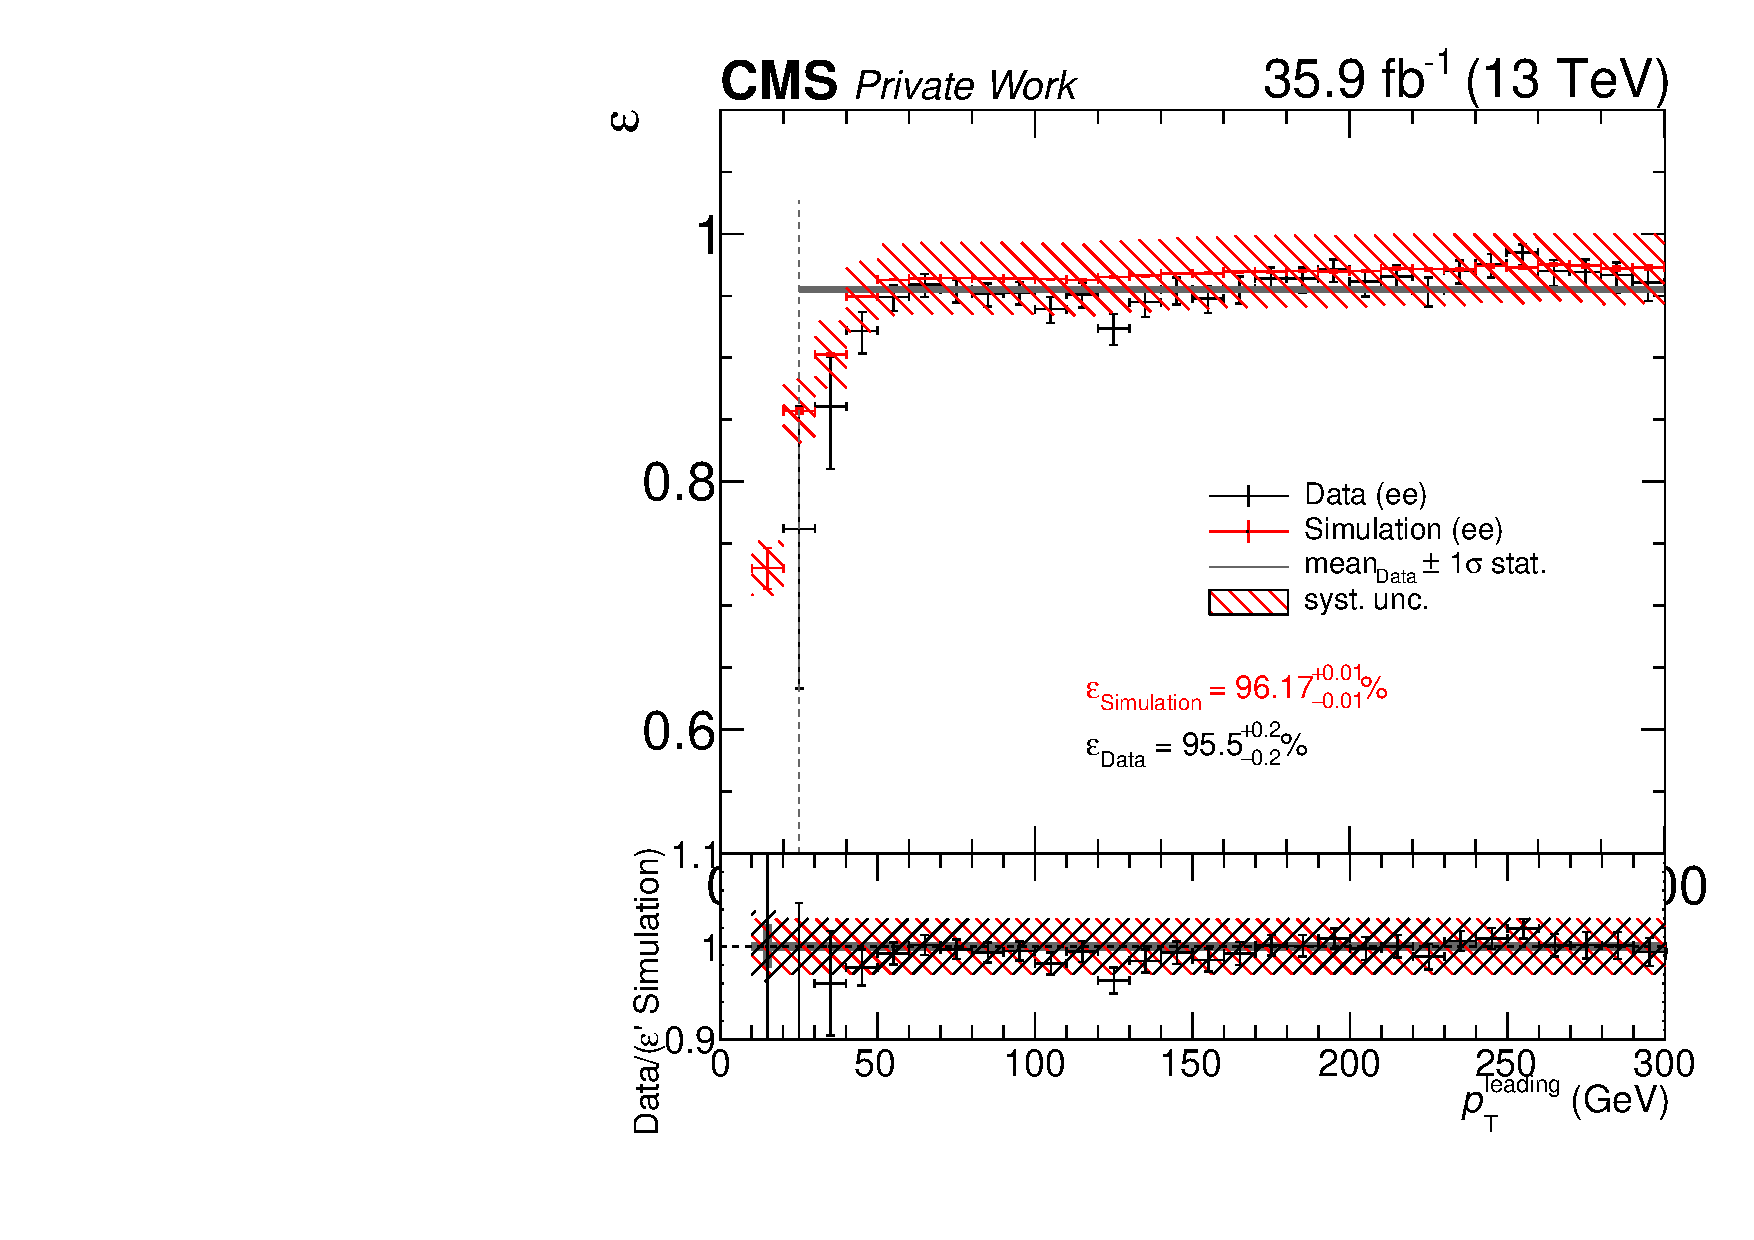
\includegraphics[width=\pairwidth]{figures/triggerStudies/efficiency_dataHT_trigDilep_EE_pt1}
 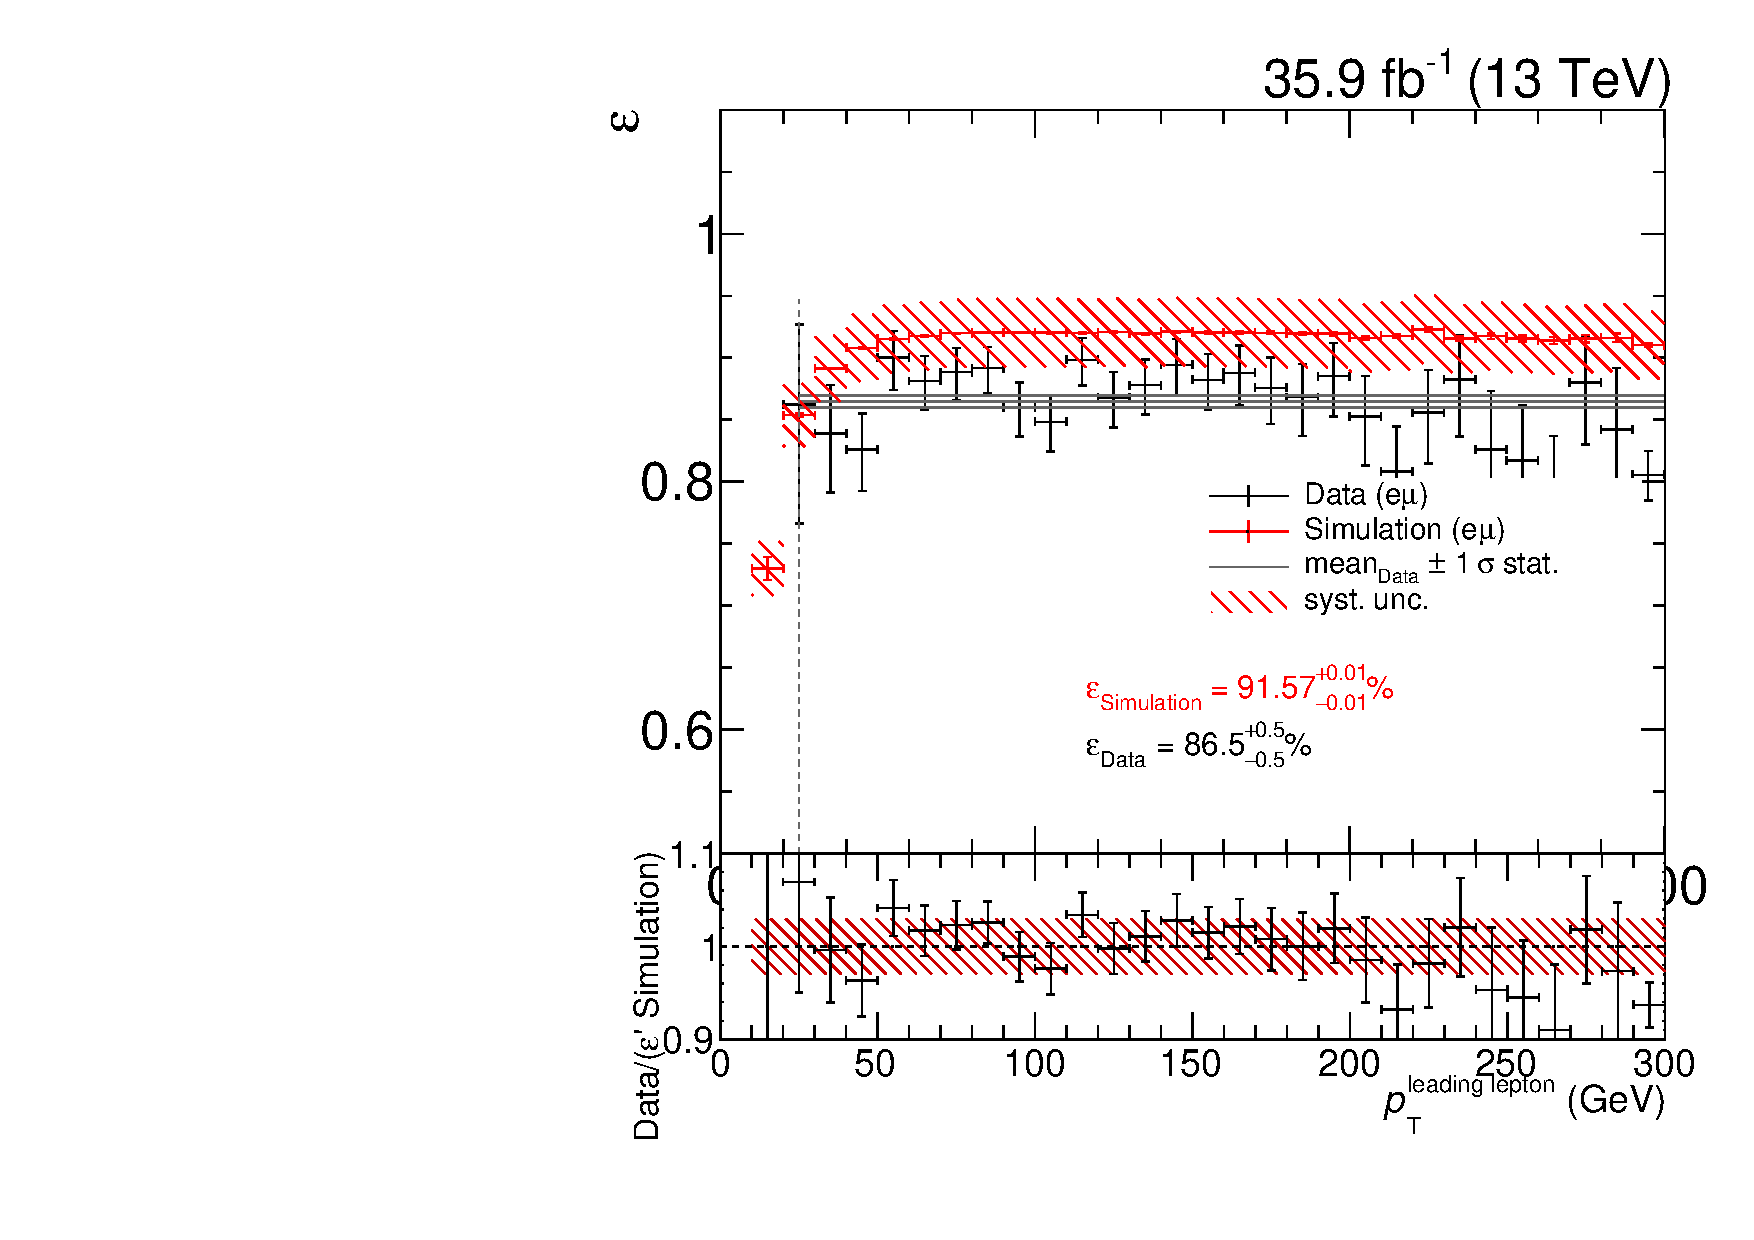
\includegraphics[width=\pairwidth]{figures/triggerStudies/efficiency_dataHT_trigDilep_EM_pt1}
 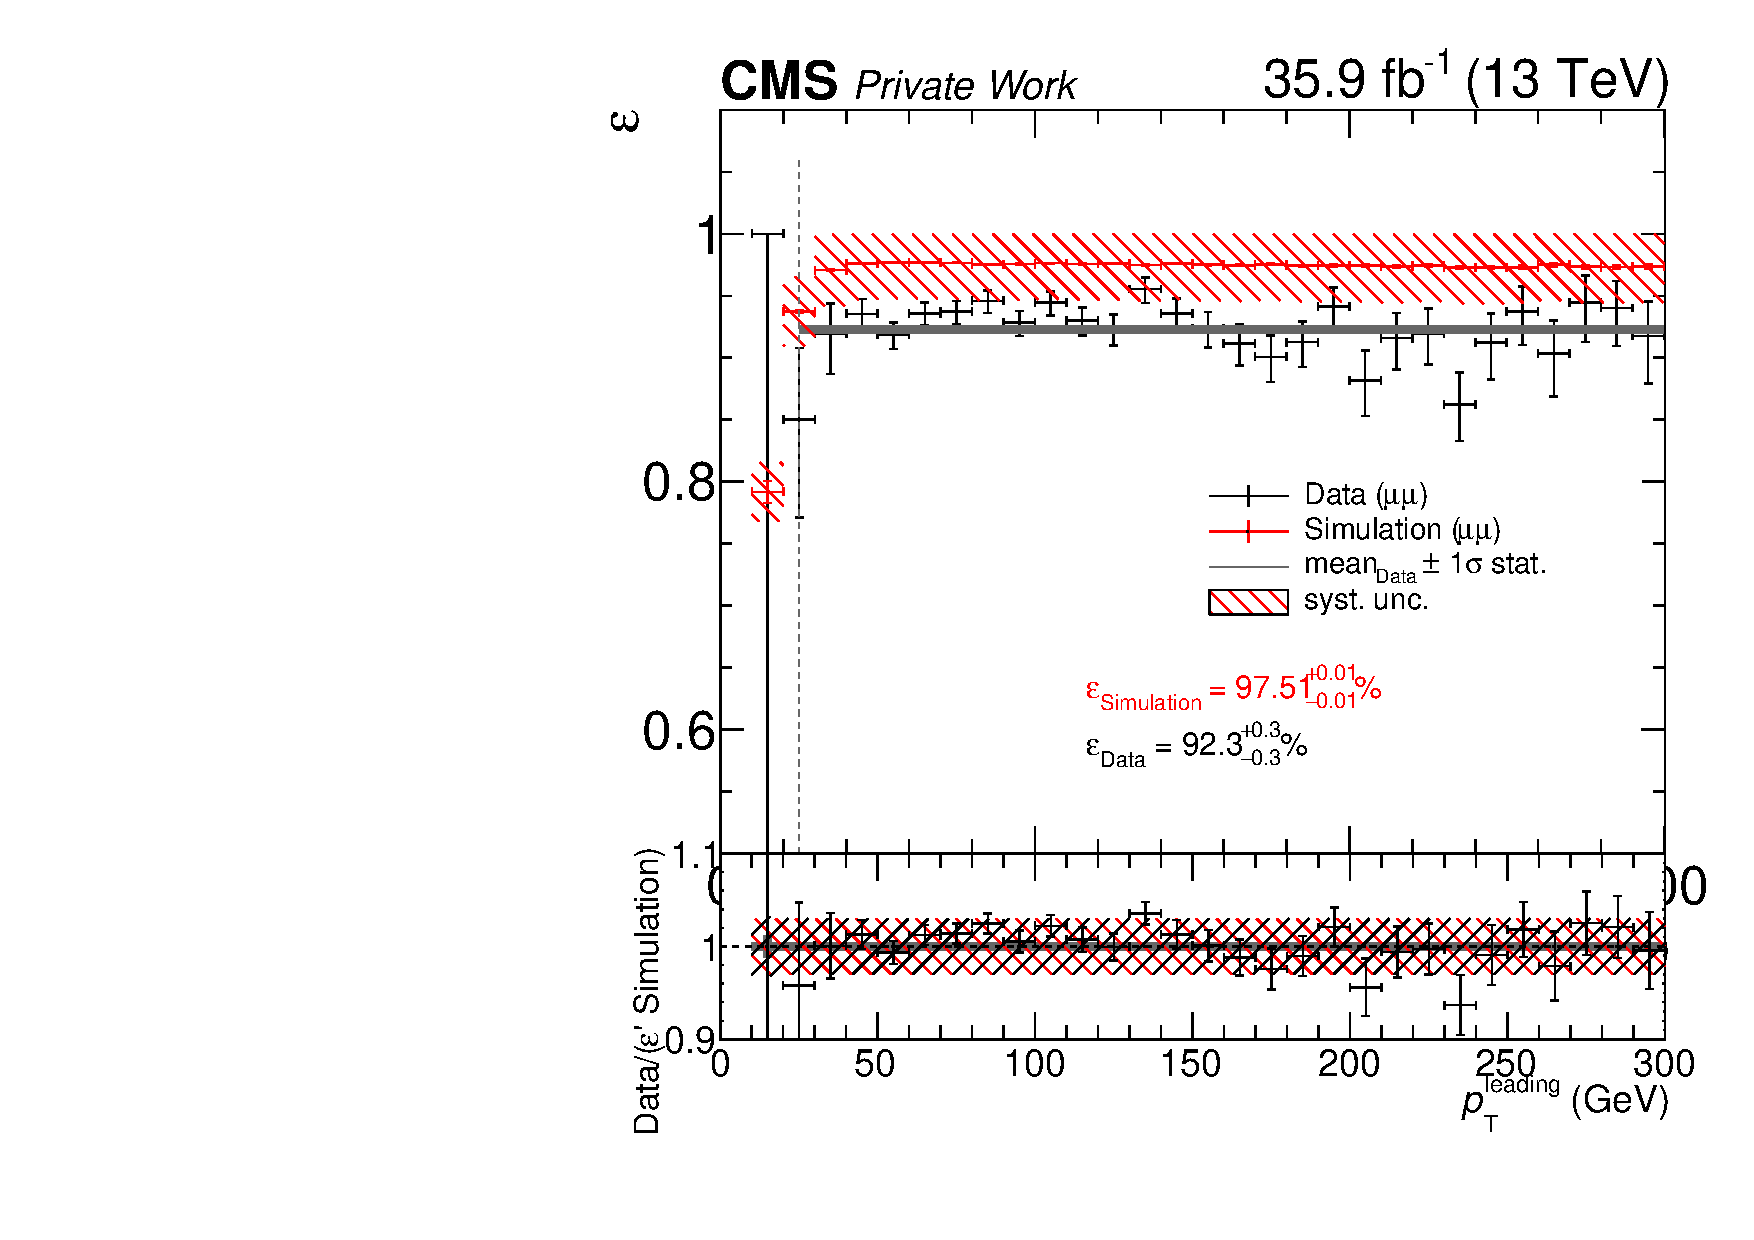
\includegraphics[width=\pairwidth]{figures/triggerStudies/efficiency_dataHT_trigDilep_MM_pt1}
 \caption{Measurement of the combined efficiency in the $\pt$ distribution of the leading lepton for all dilepton trigger combinations on data (black) and simulation (red) for the $\Pe\Pe$ (top left), $\Pe\PGm$ (top right), and $\PGm\PGm$ (bottom) channels. The measurement is performed using various $\HT$ baseline triggers, while the selection consists of the lepton pair preselection, and a $\HT>200\GeV$ requirement. The mean of the data efficiency with its statistical uncertainty (gray band), and the $3\%$ systematic uncertainty on the measurement (red band) are also shown. In the bottom panel of each plot, the ratio between the efficiency measured on data and the simulation scaled with the reweighting factor $\varepsilon'$ is shown.}
 \label{fig:app_triggEff}
\end{figure}

\begin{figure}[htb]
 \centering
 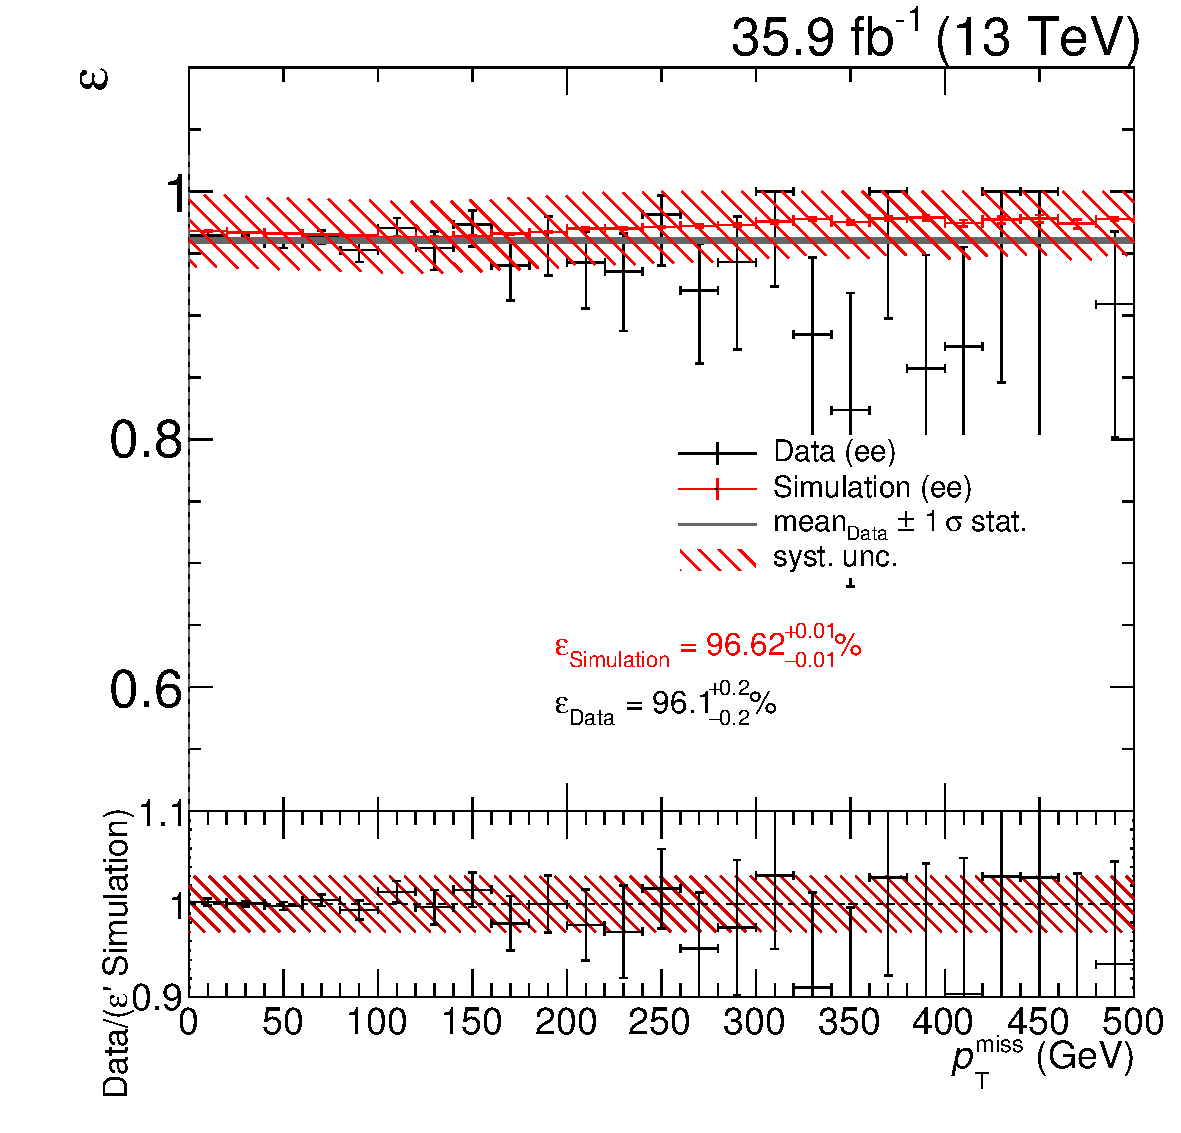
\includegraphics[width=\pairwidth]{figures/triggerStudies/efficiency_dataHT_trigDilep_ptcuts_EE_met}
 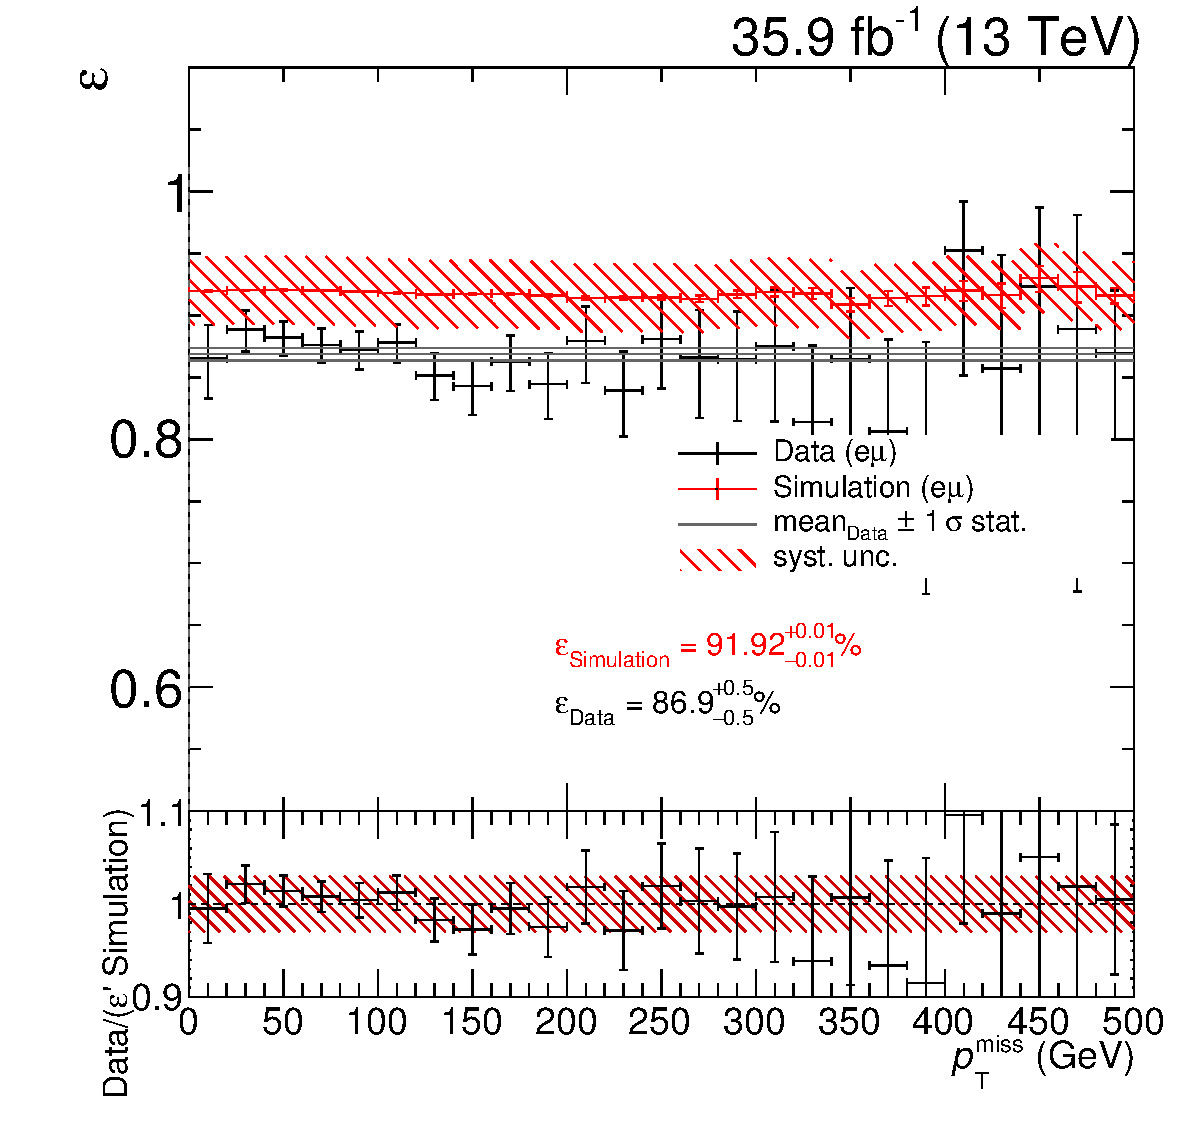
\includegraphics[width=\pairwidth]{figures/triggerStudies/efficiency_dataHT_trigDilep_ptcuts_EM_met}
 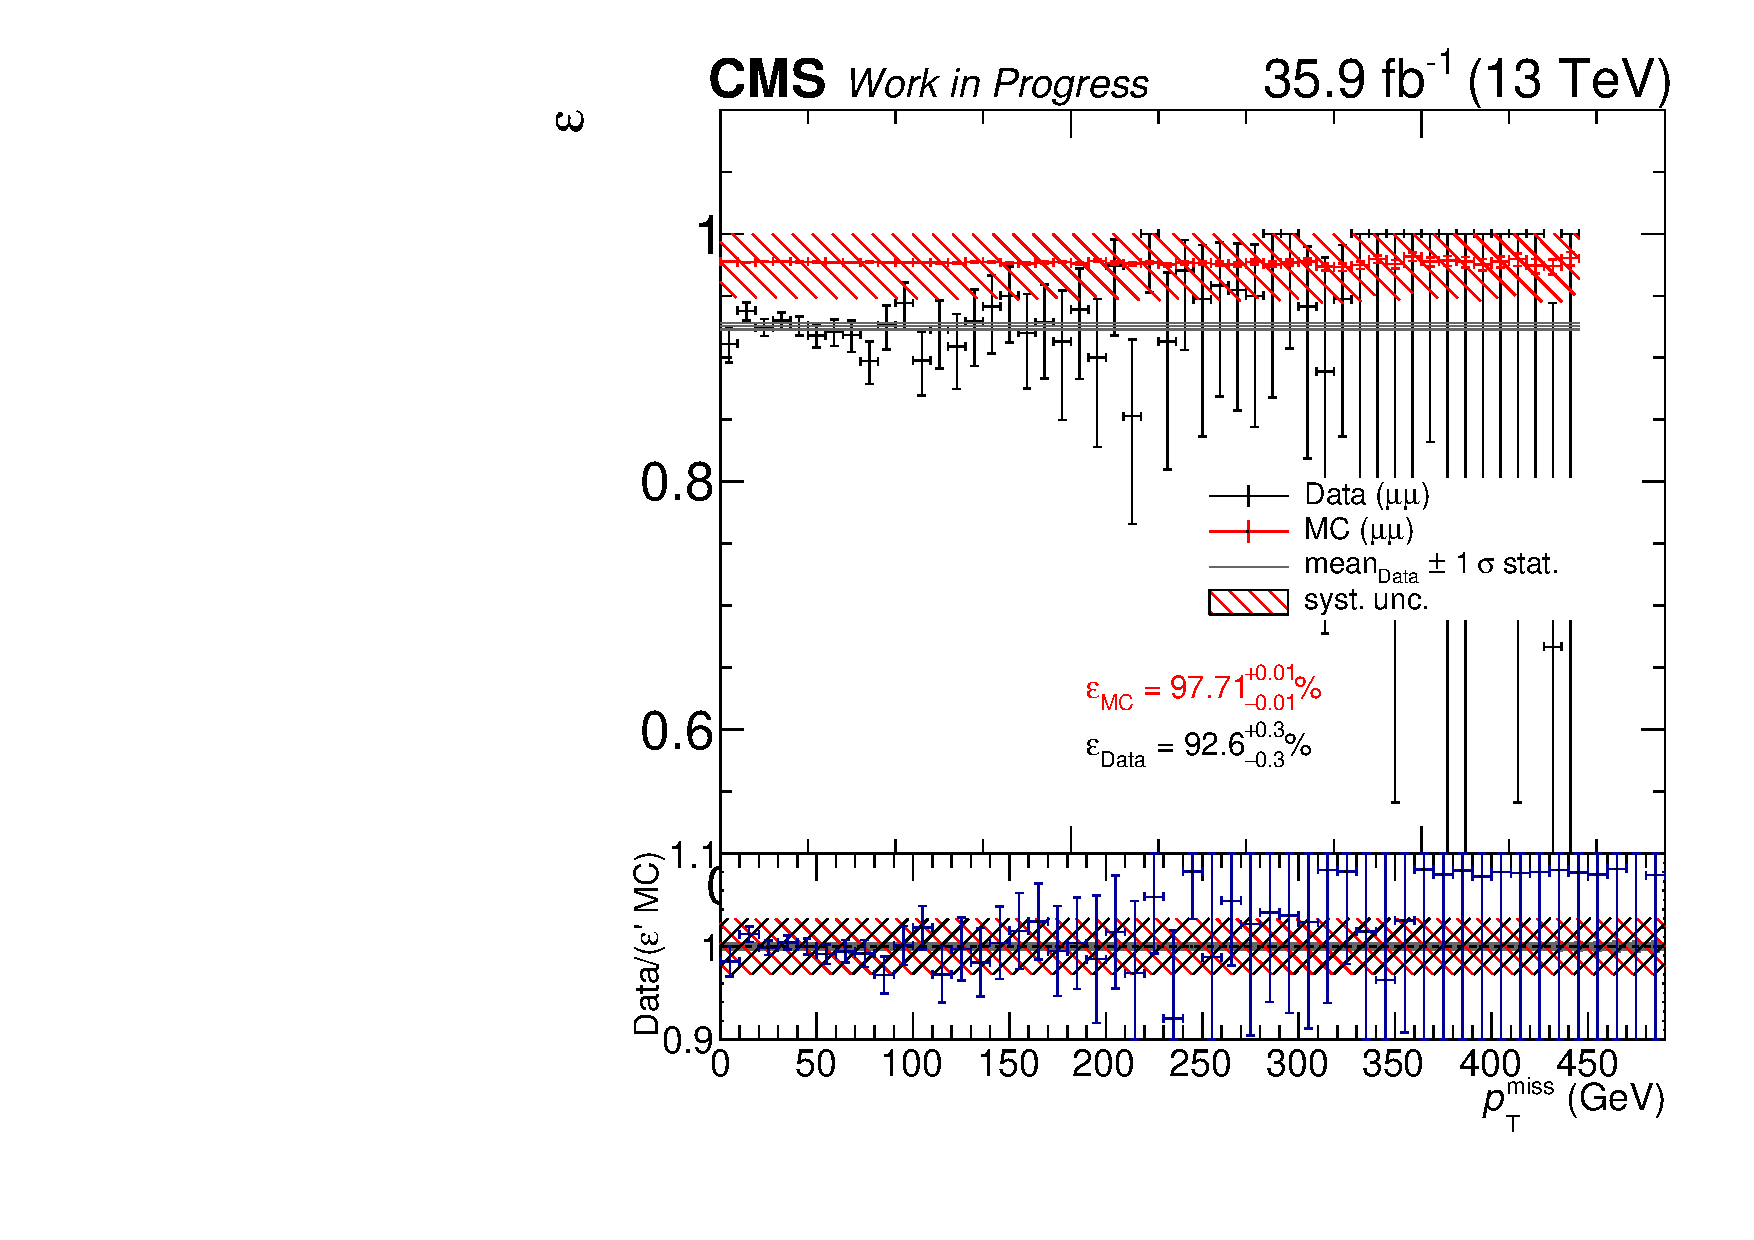
\includegraphics[width=\pairwidth]{figures/triggerStudies/efficiency_dataHT_trigDilep_ptcuts_MM_met}
 \caption{Measurement of the combined efficiency in the $\ptmiss$ distribution for all dilepton trigger combinations on data (black) and simulation (red) for the $\Pe\Pe$ (top left), $\Pe\PGm$ (top right), and $\PGm\PGm$ (bottom) channels. The measurement is performed using various $\HT$ baseline triggers, while the selection consists of the lepton pair preselection, and a $\HT>200\GeV$ requirement. The mean of the data efficiency with its statistical uncertainty (gray band), and the $3\%$ systematic uncertainty on the measurement (red band) are also shown. In the bottom panel of each plot, the ratio between the efficiency measured on data and the simulation scaled with the reweighting factor $\varepsilon'$ is shown.}
 \label{fig:app_triggEff2}
\end{figure}

\begin{figure}[htb]
 \centering
 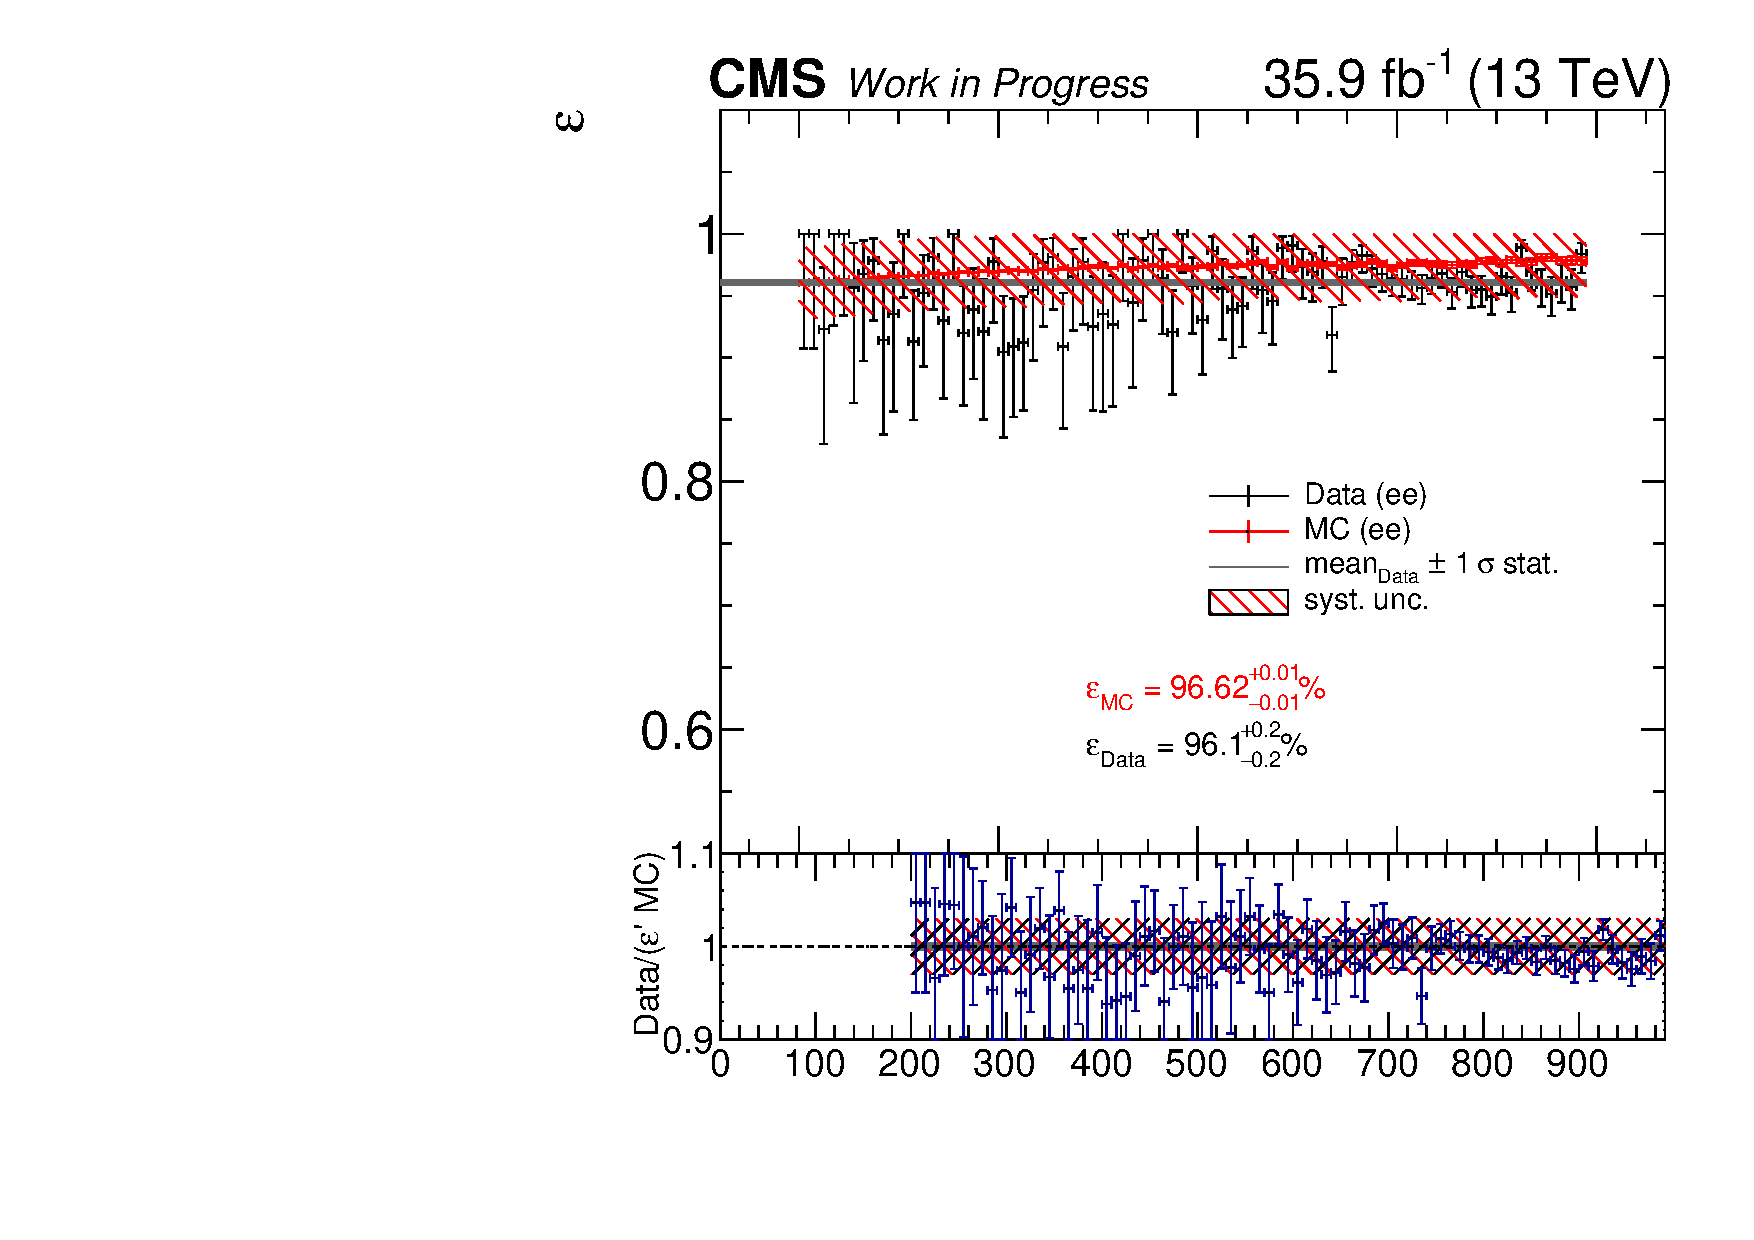
\includegraphics[width=\pairwidth]{figures/triggerStudies/efficiency_dataHT_trigDilep_ptcuts_EE_ht}
 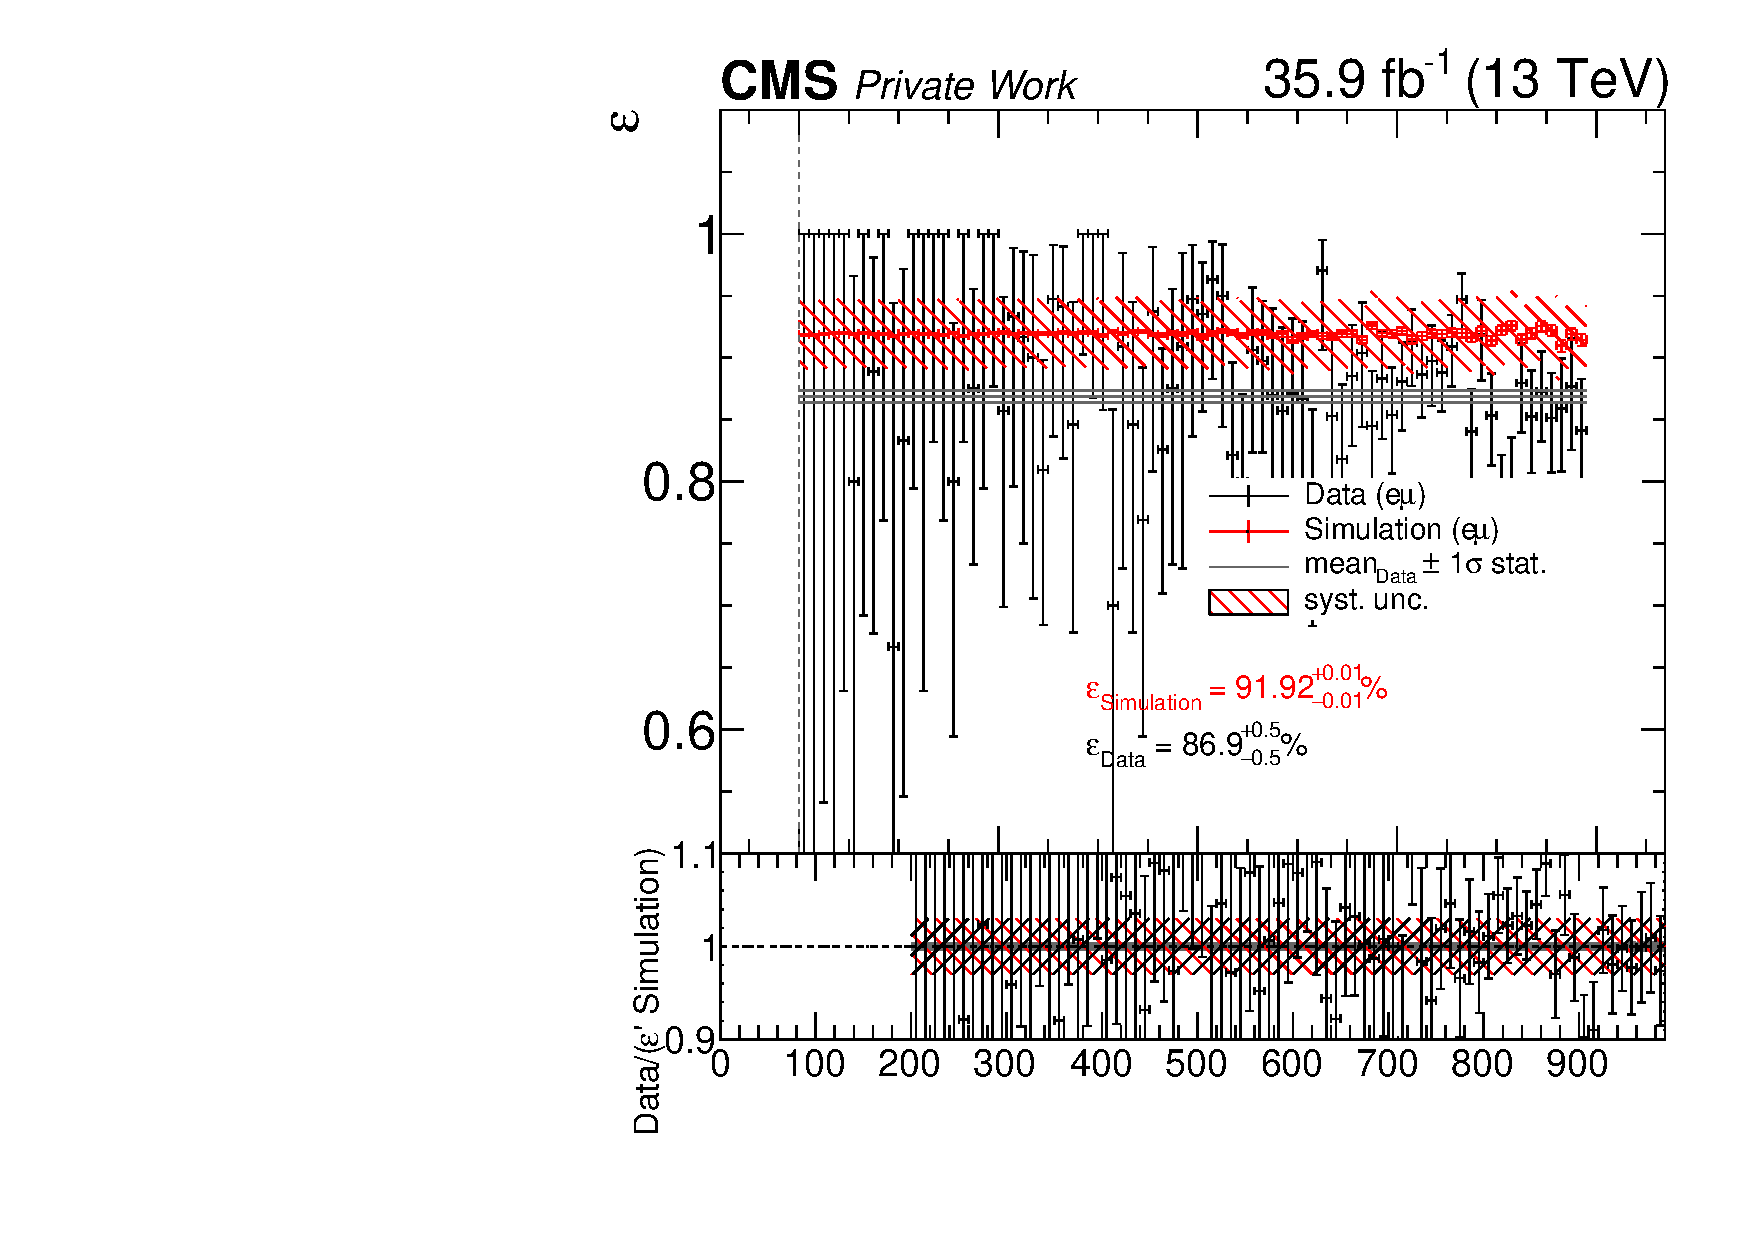
\includegraphics[width=\pairwidth]{figures/triggerStudies/efficiency_dataHT_trigDilep_ptcuts_EM_ht}
 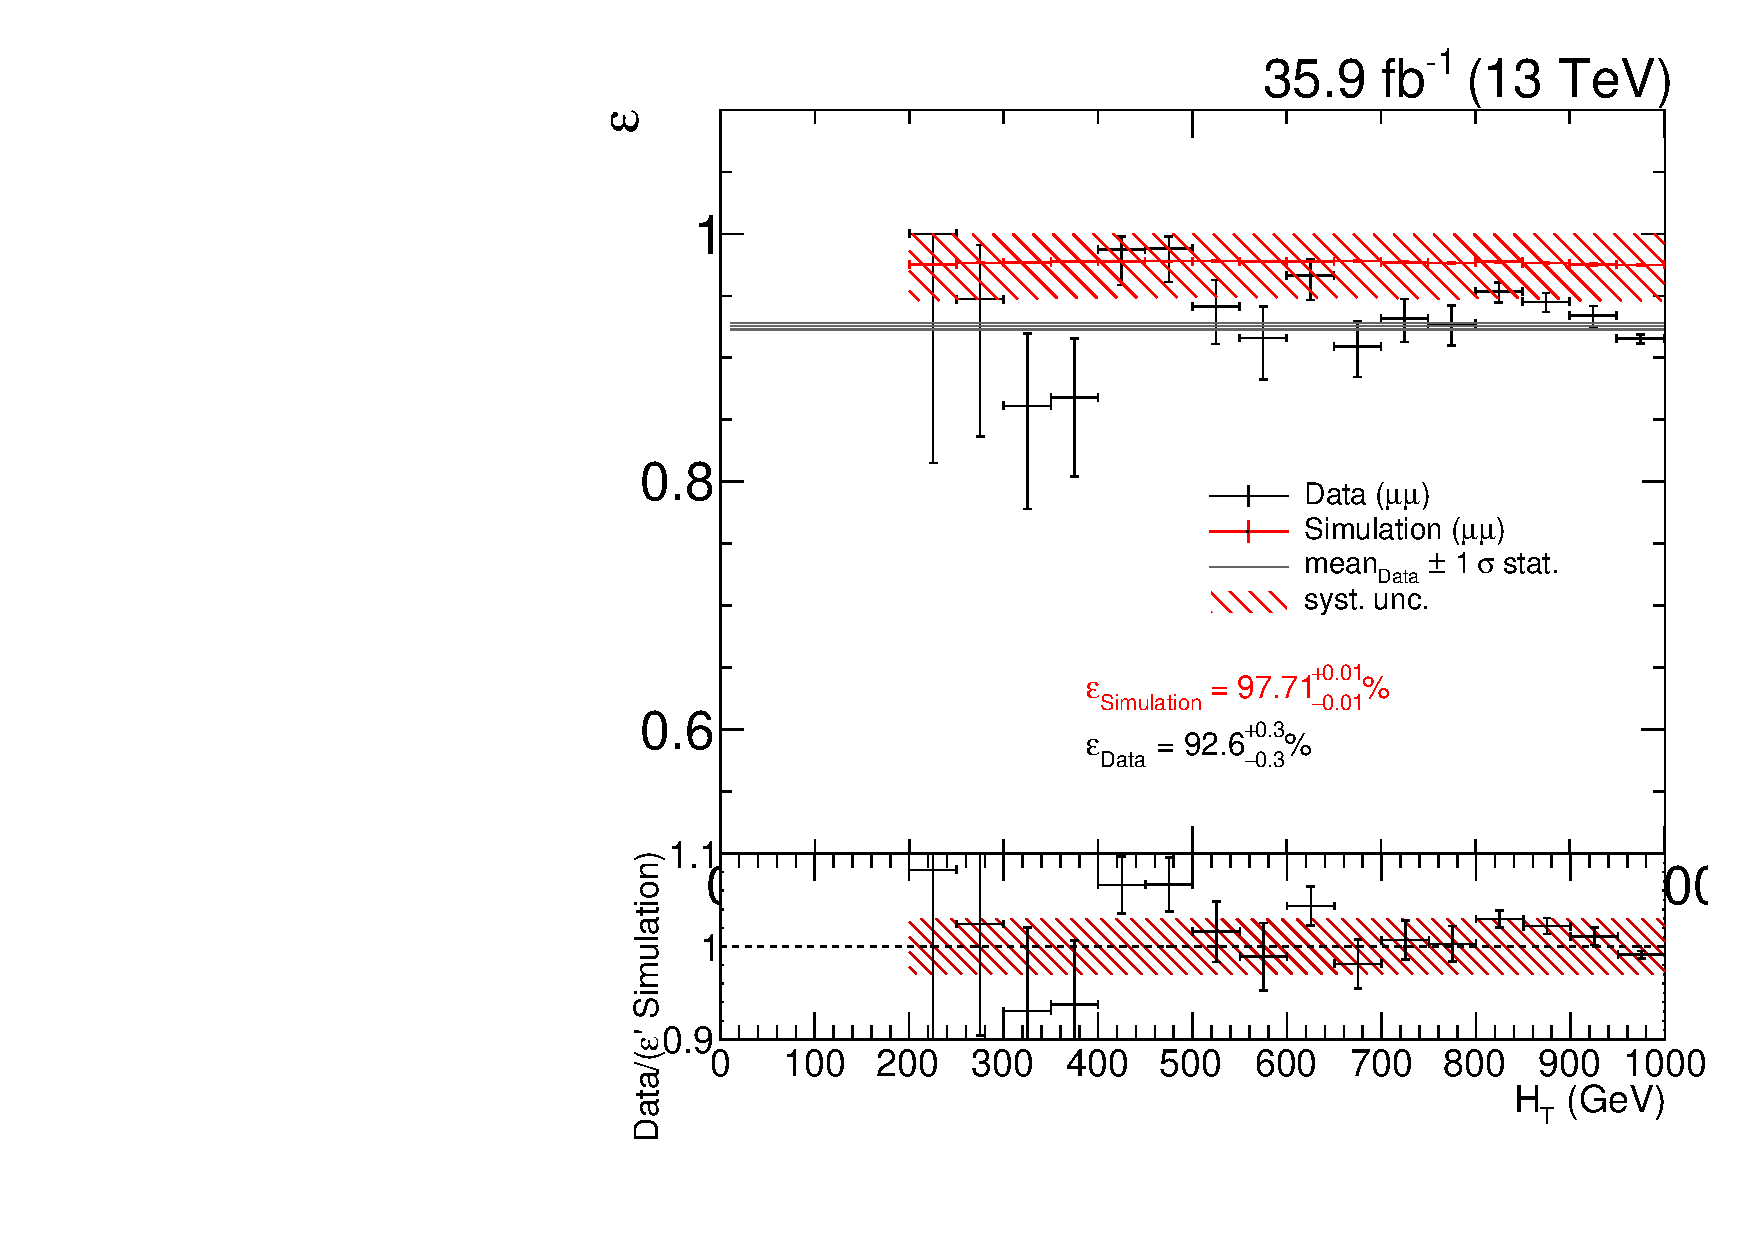
\includegraphics[width=\pairwidth]{figures/triggerStudies/efficiency_dataHT_trigDilep_ptcuts_MM_ht}
 \caption{Measurement of the combined efficiency in the $\HT$ distribution for all dilepton trigger combinations on data (black) and simulation (red) for the $\Pe\Pe$ (top left), $\Pe\PGm$ (top right), and $\PGm\PGm$ (bottom) channels. The measurement is performed using various $\HT$ baseline triggers, while the selection consists of the lepton pair preselection, and a $\HT>200\GeV$ requirement. The mean of the data efficiency with its statistical uncertainty (gray band), and the $3\%$ systematic uncertainty on the measurement (red band) are also shown. In the bottom panel of each plot, the ratio between the efficiency measured on data and the simulation scaled with the reweighting factor $\varepsilon'$ is shown.}
 \label{fig:app_triggEff3}
\end{figure}
